% path to figures directory
\graphicspath{{img/chapter_4/}}

\chapter{Models of neutrino mass and the flavour anomalies}
\label{chapter:neutrino-mass-and-flavour-anomalies}

\begin{flushleft}
  \textit{This chapter is based on the publications `Reconsidering the One
    Leptoquark scenario: flavour anomalies and neutrino mass,' written in
    collaboration with Yi Cai, Michael A. Schmidt, and Raymond R.
    Volkas~\cite{Cai:2017wry}, and `A near-minimal leptoquark model for
    reconciling flavour anomalies and generating radiative neutrino masses,'
    written with Innes Bigaran and Raymond R. Volkas~\cite{Bigaran:2019bqv}. We
    explore the tantalising connection between models of radiative neutrino mass
    and explanations of the flavour anomalies. We consider two specific models,
    and conclude with more general comments about interesting models we choose
    from our model database. We exclusively use four-component spinor notation
    in this chapter.}
\end{flushleft}

\section{Introduction}

Taken together, the flavour anomalies paint a picture of new physics interacting
more strongly with the second and third generations of SM fermions, introducing
lepton flavour non-universality and FCNC interactions at energies not
significantly higher than the electroweak scale. Interestingly, many of these
phenomenological motifs arise naturally in radiative models of neutrino mass,
hinting towards the attractive possibility of a common explanation for both
phenomena.

In Chapter~\ref{chapter:mv-models}, we presented our model database containing
all minimal tree-level $\Delta L = 2$ models. These give rise to neutrino masses
at the loop level with exotic particle content that we have already seen is
dominated by (scalar) leptoquarks. In the present chapter we explore the
relationship between the flavour anomalies and models of radiative neutrino mass
by (i) studying a radiative scenario containing the $S_{1}$ leptoquark in
detail, (ii) building a more complex model involving an additional leptoquark,
$S_{3} \sim (\mathbf{3}, \mathbf{3}, -\tfrac{1}{3})$, for a more precise
explanation of the anomalies, and (iii) commenting more generally on a more
systematic approach to studying the possible relationship between the anomalies
and radiative models of Majorana neutrino mass.

Previous work has also considered radiative neutrino mass models whose particle
content addresses the $b \to s$ anomalies, $R_{D^{(*)}}$, and $(g-2)_\mu$,
\textit{e.g.}~\cite{Pas:2015hca, Cheung:2016fjo, Cheung:2017efc, Cheung:2016frv,
  Popov:2016fzr, Deppisch:2016qqd, Babu:2010vp}. In Refs.~\cite{Pas:2015hca,
  Deppisch:2016qqd} the flavour anomalies are explained through two light scalar
or vector leptoquarks whose couplings to the SM Higgs doublet and fermions
prohibit a consistent assignment of lepton number to the leptoquarks such that
the symmetry is respected. Thus $\mathrm{U}(1)_L$ is explicitly broken by two
units and the neutrinos gain mass at the one-loop
level~\cite{AristizabalSierra:2007nf}, apart from the imposition of any
additional symmetries\footnote{Mass generation in Ref.~\cite{Babu:2010vp} occurs
  at the two-loop level because the Yukawa couplings of one of the leptoquarks
  to the left-chiral fermions is turned off.}. A general feature of such models
is that large amounts of fine-tuning are required to suppress the neutrino mass
to the required scale with at least one set of leptoquark--fermion couplings
sizeable enough to explain the anomalies.

\section{A minimal neutrino-mass scenario with $S_{1}$}
\label{sec:ch4-s1-mv}

\begin{figure}[t]
  \centering
  \begin{tikzpicture}
    \begin{feynman}
      \vertex (a) {$\nu$};
      \vertex [right=4em of a] (b);
      \vertex [right=5em of b] (c);
      \vertex [right=5em of c] (d);
      \vertex [right=4em of d] (e) {$\nu$};
      \vertex [above=5em of c] (v);
      \diagram* {
        (a) -- [fermion] (b) -- [anti charged scalar, edge label'=$S_{1}^{a}$] (c) -- [fermion, edge label'=$b$] (d) -- [anti fermion] (e),
        (b) -- [anti fermion, quarter left, edge label=$b$] (v) -- [charged scalar, quarter left, edge label=$S_{1}^{a}$] (d),
        (c) -- [majorana, edge label'=$f$] (v),
      };
    \end{feynman}
  \end{tikzpicture}
  \caption[Two loop neutrino mass generation in the model of
  Ref.~\cite{Angel:2013hla}.]{Two loop neutrino mass generation in the model of
    Ref.~\cite{Angel:2013hla}. For simplicity we consider the case where the
    leptoquark $S_{1}$ couples significantly only to the third generation of
    quarks. At least two flavours of $S_{1}$ are required to meet the neutrino
    data.}
  \label{fig:ch4-neutrinomass}
\end{figure}

In this section we incorporate the BN leptoquark into a two-loop neutrino mass
model also containing the colour octet Majorana fermion
$f \sim (\mathbf{8}, \mathbf{1}, 0)$. The model can be derived as a tree-level
completion of $\mathcal{O}_{11b} = LLQ\bar{d}Q\bar{d}$, in the notation of
Table~\ref{tab:long}. The model has been studied in detail apart from the
anomalies in Ref.~\cite{Angel:2013hla}. We summarise the key features of the
model below, and point the reader to this paper for more detail.

Following Ref.~\cite{Angel:2013hla} we couple the leptoquark $S_{1}$ to the
Majorana fermion $f$ in order to introduce the lepton-number violating terms
$m_f f f$ and $w_r \bar{d}_r f S_{1}$. The neutrino mass is proportional to the
product of down-type quark mass matrices, which is dominated by the bottom quark
mass. We do not consider the case where a strong hierarchy in the $w_r$
undermines this dominance, and thus only the coupling to the third generation of
quarks ($w_3$) is important for the neutrino mass generation. For this reason we
set $w_{1,2} = 0$ to simplify the calculation of the neutrino mass. In this
limit the neutrino mass matrix will have unit rank and an additional generation
of the leptoquark $s_{1}$ is needed to satisfy current oscillation data.
Replacing $S_{1}$ with\footnote{We highlight to the reader a redundancy in our
  notation: here we use $a, b, \ldots$ to label the leptoquark generations, not
  as colour indices, since these play no role in the discussion of this
  section.} $S_{1}^{a} = (S^{1}_1, S_1^{2})$ in Eq.~\eqref{eq:ch3-Lagra}, small
neutrino masses are generated through the two-loop graph shown in
Fig.~\ref{fig:ch4-neutrinomass} and the neutrino mass is given by
\begin{equation}
  \label{eq:ch4-massformula}
  M_{ij} \approx 4\frac{m_f
    m_b^2}{(2\pi)^8} \sum_{a, b}^2 (x_{i3a} w_{3a}) I_{ab}
  (x_{j3b} w_{3b}),
\end{equation}
where $\mathbf{I}$ is the matrix of loop integrals in the leptoquark-generation
space whose explicit form can be found in Ref.~\cite{Angel:2013hla}. This
expression for the mass matrix can be solved for the $x_{r3a}$ through the
Casas--Ibarra procedure~\cite{Casas:2001sr} to give
\begin{equation}
  \label{eq:ch4-ci}
  x_{r3a} = \frac{(2\pi)^4}{2w_{3a}m_b\sqrt{m_f}} U^*_{rs} [\tilde{\mathbf{M}}^{1/2}]_{st} R_{tb} [\tilde{\mathbf{I}}^{-1/2}\mathbf{S}]_{ba},
\end{equation}
where tildes denote real and positive diagonal matrices, $\mathbf{S}$
diagonalises the matrix $\mathbf{I}$ and $m_{b}$ is the mass of the bottom
quark. We use the best-fit values from the NuFIT collaboration for the neutrino
mixing angles and mass-squared differences~\cite{Esteban:2016qun, nufitweb},
shown in Fig.~\ref{fig:ch1-nufit-results}. The mass-squared differences fix the
elements of $\tilde{\mathbf{M}}$, since the lightest neutrino in this model is
almost massless. In the cases of normal and inverted neutrino mass hierarchy:
\begin{equation} \label{eq:ch4-r}
  \mathbf{R}^{\textsc{NO}} = \begin{pmatrix} 0 & 0\\ \cos\theta & -\sin\theta \\ \sin\theta & \cos\theta\end{pmatrix}, \quad
  \mathbf{R}^{\textsc{IO}} = \begin{pmatrix} \cos\theta & -\sin\theta \\ \sin\theta & \cos\theta \\ 0 & 0 \\\end{pmatrix},
\end{equation}
and $\theta \in \mathbb{C}$ parameterises the leptoquark--fermion Yukawa
couplings through Eq.~\eqref{eq:ch4-ci} in such a way that the correct pattern of
neutrino masses and mixings is produced. Here we consider the region of
parameter space where $m_{S_{1}^2} , m_{f} \gg m_{S_{1}^1}$ so that $S_1^{1}$
comes to be identified as the BN leptoquark, while $S_{1}^2$ and $f$ are
effectively divorced from the flavour anomalies. For this reason we refer to
$S_{1}^{1}$ simply as $S_{1}$ and suppress the leptoquark-flavour indices for
the remainder of the discussion unless a distinction is necessary. The limit
$m_{S_{1}^1} \ll m_{S_{1}^{2}}$ also allows for a simplification in the matrix
product $\tilde{\mathbf{I}}^{-1/2}\mathbf{S}$ featuring in Eq.~\eqref{eq:ch4-ci}:
\begin{equation}
  \tilde{\mathbf{I}}^{-1/2}\mathbf{S} \approx I_{11}^{-1/2} \begin{pmatrix} -i & i/\epsilon \\ 1 & \epsilon \\ \end{pmatrix},
\end{equation}
where $\epsilon \equiv I_{12}/I_{11} \ll 1$. This flavour structure implies that its
contribution to neutrino mixing is small, and thus the PMNS parameters are
principally determined by the Yukawa couplings $x_{r3a}$. We exploit this
relative insensitivity to $m_f$ and $m_{S_{1}^{2}}$ to simplify our analysis in
the following.

The decoupling of $f$ and $S_{1}^{2}$ from the relevant flavour physics makes
$w_3$ an effectively free parameter that acts as a lepton-flavour-blind scaling
factor on the couplings of the leptoquark to the third generation of quarks,
while $\theta$ governs their relative sizes for a given leptoquark flavour. We
plot the $x_{i3}$ against real $\theta$ values in Fig.~\ref{fig:ch4-xi3plot} for
the mass choices $m_f = 25 \text{ TeV}$, $m_{S_{1}^{2}} = 20 \text{ TeV}$ and
$m_{S_{1}^{1}} = 4 \text{ TeV}$ with fixed $w_3 = 0.003$. Both the normal and
inverted hierarchies are considered.

\begin{figure}[t]
  \centering%
  \begin{minipage}[t]{0.45\linewidth}
    \centering 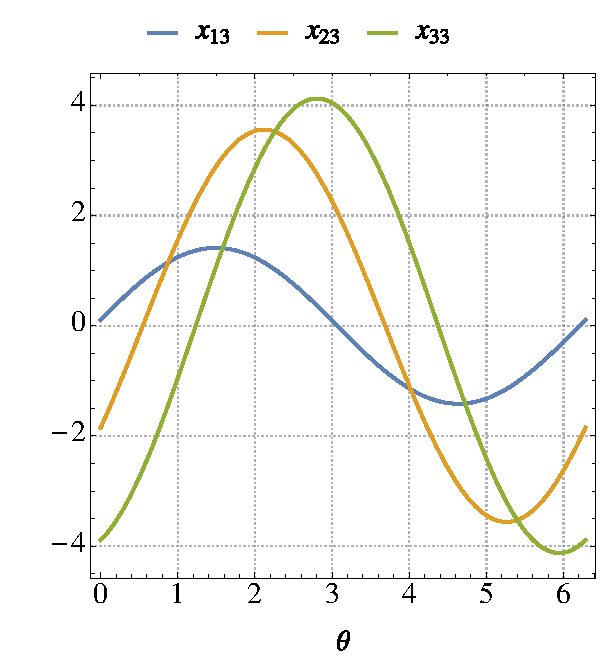
\includegraphics[scale=0.55]{xi3Plot.pdf}
    \subcaption{Normal neutrino mass hierarchy.}
    \label{fig:noxi3plot}
  \end{minipage}
  \hfill
  \begin{minipage}[t]{0.45\linewidth}
    \centering 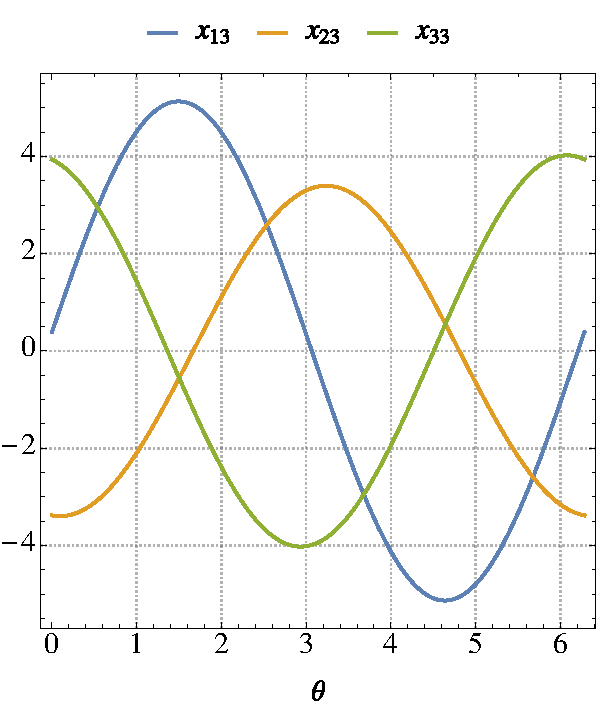
\includegraphics[scale=0.51]{xi3PlotIO.pdf}
    \subcaption{Inverted neutrino mass hierarchy.}
    \label{fig:ioxi3plot}
  \end{minipage}
  \caption{Plots of the relative sizes of the couplings of the leptoquark
    $S_{1}^{1}$ to the bottom quark and the $r$th neutrino flavour against
    $\theta$, the Casas--Ibarra parameter, for $m_f = 25 \text{ TeV}$,
    $m_{S_{1}^{2}} = \SI{20}{\TeV}$, $m_{S_{1}^{1}} = \SI{4}{\TeV}$ and
    $w_3 = 0.003$. We only consider the case $\theta \in \mathbb{R}$ here.}
  \label{fig:ch4-xi3plot}
\end{figure}

Both Fig.~\ref{fig:ch4-xi3plot} and Eq.~\eqref{eq:ch4-ci} indicate that, with
the inclusion of neutrino mass, the couplings to the electron and
electron-neutrino cannot be turned off \textit{ad libitum}. Even a small
electron coupling $z_{13} \neq 0$ can generate dangerous contributions to
muon--electron conversion in nuclei in the presence of $z_{23} \neq 0$,
necessary for the model to alleviate the tensions in the $b \to s$ transition.
We plot the current limit from muon--electron conversion experiments in gold
nuclei
$\text{Br}(\mu \ce{^{197}_{79}}\text{Au} \to e \ce{^{197}_{79}}\text{Au}) < 7.0 \cdot 10^{-13}$~\cite{Olive:2016xmw}
against $\theta$ and $w_3$ in Fig.~\ref{fig:ch4-muNeN} for both the normal and
inverted hierarchies and a range of masses $m_{S_{1}^{1}}$. The prospective
limit from the COMET experiment: $\text{Br} \sim 10^{-16}$~\cite{Kurup:2011zza},
is also shown. A fit to the neutrino oscillation data while respecting
measurements of muon--electron conversion implies a fine-tuning in
$\theta$---or, equivalently, $z_{31}$---to arrange $|z_{31}| \ll |z_{33}|$,
pushing the model into a very specific region of parameter space. The required
$x_{31} \approx 0$ can be arranged with $\theta \approx 3.08 \pm n\pi$, fixing
the ratio $x_{33}/x_{32} = 1.96$ for the normal neutrino mass hierarchy, and
$x_{33}/x_{32} = -0.85$ for the inverted hierarchy. Comparison with
Fig.~\ref{fig:ch3-x33x32rat}, however, indicates that neither of the
aforementioned ratios can allow large contributions to $C_{LL}$ in the correct
direction, although the inverted hierarchy does slightly better than the normal
mass ordering. This makes a combined explanation of the $b \to s$ anomalies and
neutrino mass in this model problematic. If, instead, one required that this
model explain $R_{D^{(*)}}$, $(g-2)_\mu$ and neutrino mass, the values of
$x_{33}$ required are compatible with both the normal and inverted hierarchies,
and the model remains agnostic with respect to its preference.

\begin{figure}[t]
  \centering
  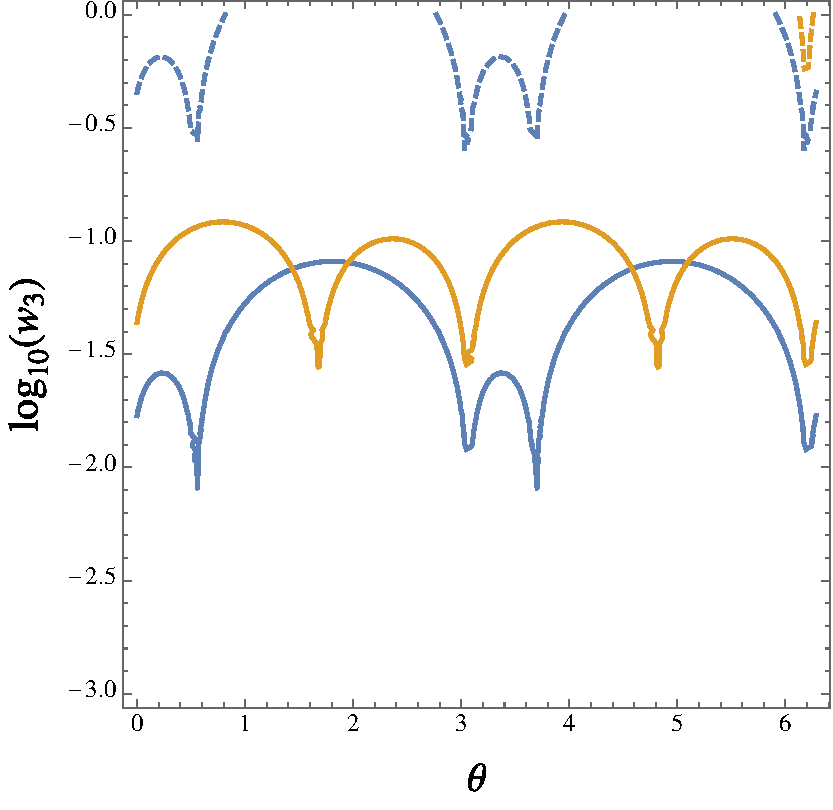
\includegraphics[scale=0.45]{muNeN}
  \caption[The figure shows the current (solid) and
  expected~\cite{Kurup:2011zza} (dashed) limits from muon--electron conversion
  in nuclei in the $\theta$--$w_3$ plane for normal mass ordering (blue) and
  inverted ordering (orange).]{The figure shows the current (solid) and
    expected~\cite{Kurup:2011zza} (dashed) limits from muon--electron conversion
    in nuclei in the $\theta$--$w_3$ plane for normal mass ordering (blue) and
    inverted ordering (orange). The region below each curve is ruled out. The
    dips at $\theta \approx 3.08$ and $\theta \approx 6.22$ stretch to negative
    infinity. Aside from accidental cancellation, the values
    $\theta \approx 3.08, 6.22$ ensure that the coupling to the electron
    vanishes. Only real values of $\theta$ are considered.}
  \label{fig:ch4-muNeN}
\end{figure}

\section{A non-minimal model: $S_{1}$ and $S_{3}$}
\label{sec:ch4-non-minimal}

In the previous chapter it was shown that the BN scenario, although powerful
given its simplicity, is restricted in its ability to adequately explain both
the neutral- and charged-current anomalies. Additionally, the simple
neutrino-mass embedding we study above is incompatible with an explanation of
the neutral-current anomalies on account of LFV effects, which must be present
in radiative neutrino-mass models. To further explore the extent to which these
LFV effects can be circumnavigated in a model of neutrino mass and the flavour
anomalies, we build a non-minimal model that also can better accommodate a
simultaneous explanation of the $b \to s$ and $b \to c$ data.

It is known that a particularly simple model that can accommodate the
neutral-current anomalies is that involving the scalar isotriplet leptoquark
$S_{3} \sim (\mathbf{3}, \mathbf{3}, -\tfrac{1}{3})$~\cite{Hiller:2014yaa,
  Kumar:2018era}. The field mediates the $b \to s \mu\mu$ interaction at
tree-level, and $C_{LL} \simeq -1.0$ can be accommodated in the face of almost
no other constraints. It is also clear from Fig.~\ref{fig:ch3-money1} that the
BN leptoquark with contributions along the scalar--tensor direction can explain
$R_{D^{(*)}}$ to within the $1\sigma$ region of the combined fit. Thus, it seems
sensible to construct a radiative neutrino-mass model containing both the
$S_{1}$ and $S_{3}$ leptoquarks in the hope that the LFV bounds can be
alleviated with the increased parameter choices. The operator analysis presented
in Chapter~\ref{chapter:mv-models}, along with other similar
approaches~\cite{Cai:2014kra, Bonnet:2012kz, Klein:2019iws}, finds two UV models
derived from the dimension-seven operators $\mathcal{O}_{3a,b}$ that contain
these fields, shown in Table~\ref{tab:ch4-d7-models}. In the following we study
the combined model that contains the three fields $S_{1}$, $S_{3}$ and the vector-like fermion
\begin{equation}
  \chi_{L,R} \sim (\mathbf{3}, \mathbf{2} - \tfrac{5}{6})
\end{equation}
with the intention that $S_{1}$ explain $R_{D^{(*)}}$ at tree-level, $S_{3}$
explain the $b \to s$ data at tree-level, and $\chi_{L,R}$ participate in the
neutrino-mass mechanism. Our aim is to explore the extent to which this
next-to-minimal model can accommodate neutrino masses, the flavour anomalies and
bounds from LFV processes, as a representative example.

\begin{table}[t]
  \centering
  \bgroup
  \def\arraystretch{1.3}
  \begin{tabular}{cc}
    \toprule
    Model 1 & Model 2 \\
    \midrule
    $S_{3} \sim (\mathbf{3}, \mathbf{3}, -\tfrac{1}{3})$ & $S_{1} \sim (\mathbf{3}, \mathbf{1}, -\tfrac{1}{3})$\\
    $\chi_{L,R} \sim (\mathbf{3}, \mathbf{2}, -\tfrac{5}{6})$ & $\chi_{L,R} \sim (\mathbf{3}, \mathbf{2}, -\tfrac{5}{6})$\\
    \bottomrule
  \end{tabular}
  \egroup
  \caption[Particle content of two radiative models derived from dimension-seven
    operators identified in our model
    database~\cite{gargalionis_john_2020_4054618} that contain $S_{1}$ and
    $S_{3}$.]{Particle content of two radiative models derived from dimension-seven
    operators identified in our model
    database~\cite{gargalionis_john_2020_4054618} that contain $S_{1}$ and
    $S_{3}$. Both models contain the vector-like quark $\chi_{L} + \chi_{R}$
    whose components mix into the bottom quark.}
  \label{tab:ch4-d7-models}
\end{table}

\subsection{The model}
\label{sec:ch4-innes-model}

The combination of models 1 and 2 of Table.~\ref{tab:ch4-d7-models} provides a particle content of
\begin{align*}
\chi_{L} \sim (\textbf{3}, \textbf{2}, -\tfrac{5}{6})_{(\mathbf{2}, \mathbf{1})} \ , \, \chi_{R} \sim (\textbf{3}, \textbf{2}, -\tfrac{5}{6})_{(\mathbf{1}, \mathbf{2})} \ , \,
S_{1} \sim ({\textbf{3}}, \textbf{1}, -\tfrac{1}{3})_S \ , \, S_{3} \sim  (\textbf{3}, \textbf{3}, -\tfrac{1}{3})_S
\end{align*}
for the model. The extension to the SM Lagrangian is
$\Delta \mathscr{L} = \mathscr{L}_{\text{int}} + \mathscr{V}$, where
\begin{equation}
  \label{eq:ch4-int-lag}
  \mathscr{L}_{\text{int}} = m_{\chi} \bar{\hat{\chi}}_{L} \hat{\chi}_{R} + \hat{x}_{d} \bar{\hat{d}}_{R} H \hat{\chi}_{L} + (\hat{x}_{1} S_{1}^{\dagger} - \hat{x}_{3} S_{3}^{\dagger}) \hat{L} \hat{Q} + \hat{y} \hat{e}_{R} \hat{u}_{R} S_{1} + (\hat{w}_{1} S_{1} - \hat{w}_{3} S_{3}) \bar{\hat{\chi}}_{R} \hat{L} + \text{h.c.}
\end{equation}
and the potential is
\begin{equation}
  \label{eq:ch4-potential}
  \begin{aligned}
    -\mathscr{V} &= \sum_{a \in \{1, 3\}} \left(m_{S_{a}}^{2} |S_{a}|^{2} + \lambda_{a} |S_{a}|^{4} + \lambda_{Ha} |S_{a}|^{2} |H|^{2}\right) + \lambda_{13} |S_{1}|^{2} |S_{3}|^{2} + \lambda_{H3}^{\prime} |S_{3} H|^{2} \\
    &\quad + (\kappa H S_{1} H^{\dagger} S_{3}^{\dagger} + \text{h.c.}) \ .
  \end{aligned}
\end{equation}
Here again, we use hats to indicate interaction-eigenstate fields. Isospin,
colour and flavour indices have been suppressed, and we use $a$ to index the
leptoquark types. The last term in the potential leads to a mixing between the
$S_{1}$ and $S_{3}$ leptoquarks, governed by $\kappa$. We choose to set all
quartic terms in the scalar potential to zero for simplicity, since they play no
role in the neutrino mass or the anomalies. As this implies $\kappa = 0$ at
least at tree-level, we show the leptoquarks as unhatted fields in
Eqs.~\eqref{eq:ch4-int-lag} and \eqref{eq:ch4-potential}. Global
$\mathrm{U}(1)_{B}$ has been imposed on the Lagrangian to prevent the
simultaneous presence of the diquark and lepton--quark couplings for both
$S_{1}$ and $S_{3}$, since these are together sufficient to mediate tree-level
proton decay. The second term in $\mathscr{L}_{\text{int}}$ leads to mixing
between the down-type quarks and $\chi$. For simplicity, we set the $x_{d}$
coupling to the first two generations of down-type quarks to zero, \textit{i.e.}
$x_{d}^{1} = x_{d}^{2} = 0$, so that there is only mixing between $\chi$ and the
bottom quark. We will see this to be motivated by the structure of the
neutrino-mass matrix in Sec.~\ref{sec:ch4-innes-neutrino-mass}. We choose to
label the $\mathrm{SU}(2)_{L}$ components of $\chi_{L,R}$
\begin{equation}
  \hat{\chi}_{X} = \begin{pmatrix} \hat{B}_{X} \\ \hat{Y}_{X} \end{pmatrix} \ ,
\end{equation}
where $X \in \{L, R\}$. The fields $\hat{B}_{L,R}$ mix with the
interaction-eigenstate bottom quark $\hat{b}_{X}$:
\begin{equation}
  \label{eq:ch4-b-mixing}
  \begin{pmatrix} b_{X} \\ B_{X} \end{pmatrix} = \begin{pmatrix}
    \cos \theta_{X} & \sin \theta_{X} \\
    -\sin \theta_{X} & \cos \theta_{X}
  \end{pmatrix}^{\dagger} \begin{pmatrix} \hat{b}_{X} \\ \hat{B}_{X} \end{pmatrix} \ ,
\end{equation}
forming the mass eigenstates $B_{X}$ and $b_{X}$. The physical masses are given by
\begin{equation}
  m_{b}^{2} = m_{\hat{b}}^{2} - m_{bB}^{2} \frac{m_{\chi}^{2}}{m_{\chi}^{2} - m_{\hat{b}}^{2}} \ ,\quad
  m_{B}^{2} = m_{\chi}^{2} + m_{bB}^{2} \frac{m_{\hat{b}}^{2}}{m_{\chi}^{2} - m_{\hat{b}}^{2}} \ ,
\end{equation}
with $m_{bB} = x_{d}^{3}v / \sqrt{2}$, $m_{\hat{b}} = y_{b} v / \sqrt{2}$, and
\begin{equation}
  \label{eq:ch4-bmixing}
  \theta_{L} = \sin^{-1} \frac{m_{bB} m_{\chi}}{m_{\chi}^{2} - m_{\hat{b}}^{2}} \ , \quad
  \theta_{R} = \sin^{-1} \frac{m_{bB} m_{\hat{b}}}{m_{\chi}^{2} - m_{\hat{b}}^{2}} \ .
\end{equation}

Using the expressions given in Eq.~\eqref{eq:ch3-smfermion-mixing}, we move from
the interaction to the charged-fermion mass basis. We again use $\breve{\nu}_{L}$ to
represent the weak-eigenstate neutrino fields. The pertinent parts of the
Lagrangian are
\begin{equation}
  \begin{split}
    \label{eq:ch4-lag-y}
    \mathscr{L} &\supset x_{1}^{rs} \breve{\nu}_L^r \hat{d}_L^s S_{1}^\dagger - [\mathbf{x}_{1} \mathbf{V}^\dagger]^{rs} e_L^r u_L^s S_{1}^\dagger + y^{rs} e_R^r u_R^s S^{\dagger}_{1} + w^{r}_{1} (\bar{Y}_{R} e_{L} + \bar{\hat{B}}_{R} \breve{\nu}_{L}) S_{1} \\
    &\quad + \frac{x^{rs}_{3}}{\sqrt{2}} \breve{\nu}^{r}_{L} d^{s}_{L} S_{3}^{1/3} + \frac{1}{\sqrt{2}} [\mathbf{x}_{3} \mathbf{V}^\dagger]^{rs} e^{r}_{L} u^{s}_{L} S_{3}^{1/3} + x^{rs}_{3} e^{r}_{L} \hat{d}^{s}_{L} S^{4/3}_{3} - [\mathbf{x}_{3} \mathbf{V}^\dagger]^{rs} \breve{\nu}^{r}_{L} u^{s}_{L} S^{-2/3}_{3} \\
    &\quad + w^{r}_{3} (\bar{Y}_{R} e^{r}_{L} - \bar{\hat{B}}_{R} \breve{\nu}^{r}_{L}) S^{-1/3}_{3} +  w^{r}_{3} \bar{\hat{B}}_{R} e^{r}_{L} S^{-2/3}_{3} + w^{r}_{3} \bar{Y}_{R} \breve{\nu}^{r}_{L}S^{4/3}_{3} + \text{h.c.}
  \end{split}
\end{equation}
and we have now dropped the hats, except on the $d^{3} = b$ and $B$ fields,
since the mixing of Eq.~\eqref{eq:ch4-b-mixing} is still to be accounted for. We
write flavour indices as superscrpts here and in the remainder of this chapter
in order to accommodate the leptoquark labels $a$ on the coupling constants
$x_{a}$ and $z_{a}$. As in Chapter~\ref{chapter:the-one-lq}, we define
\begin{equation}
  \label{eq:ch4-z-relation}
  \mathbf{z}_{a} = \mathbf{x}_{a} \mathbf{V}^{\dagger}
\end{equation}
with $a \in \{1, 3\}$ for the left-handed couplings of the leptoquarks to
up-type quarks.

\subsection{Neutrino mass}
\label{sec:ch4-innes-neutrino-mass}

In this model there are two one-loop neutrino-mass mechanisms that are \textit{a
  priori} active: one involving $S_{1}$ and $\chi_{L} + \chi_{R}$, the other
involving $S_{3}$ and $\chi_{L} + \chi_{R}$. The neutrino-mass diagrams are
shown in Fig.~\ref{fig:ch4-one-loop-diags} in a generic way. There are also
two-loop diagrams coming about from the closure of $\mathcal{O}_{8}$, generated
by the $S_{1}$ and $\chi_{L} + \chi_{R}$ model. Neutrino masses arising from
$\mathcal{O}_{8}$ are very suppressed (see Tables~\ref{tab:ch2-example-closures}
and \ref{tab:long}) and so we disregard these contributions as subdominant.

\begin{figure}[t]
  \centering
  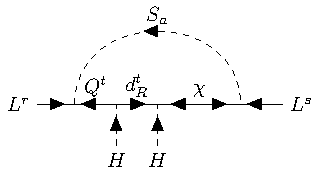
\includegraphics[width=0.5\linewidth]{ch4_neutrino_mass}
  \caption[The one-loop neutrino-mass diagrams in the combined $S_{1}$, $S_{3}$
  and $\chi_{L} + \chi_{R}$ model, shown here in the unbroken phase.]{The
    one-loop neutrino-mass diagrams in the combined $S_{1}$, $S_{3}$ and
    $\chi_{L} + \chi_{R}$ model, shown here in the unbroken phase. \textit{A
      priori} there are two neutrino-mass mechanisms operating in this model:
    one with $S_{1}$ in the loop, and another with $S_{3}$. It is clear from the
    diagram that the neutrino-mass matrix is proportional to the down-quark mass
    matrix.}
  \label{fig:ch4-one-loop-diags}
\end{figure}

We calculate these one-loop diagrams in the mass-basis, finding
\begin{equation}
  \label{eq:ch4-neutrino-mass-matrix}
  \begin{aligned}
    [\mathbf{m}_\nu]_{rs} &= \frac{3m_{B} m_b }{16\pi^2}m_{bB} \sum_{a \in \{1, 3\}}  (2 - \delta_{a3}) [x_{a}^{r3} w_{a}^s + (r \leftrightarrow s)] \frac{1}{m_{B}^2-m_{S_{a}}^2} \log \frac{m_{B}}{m_{S_{a}}} \ ,
  \end{aligned}
\end{equation}
in the sensible limit that $m_{b} \ll m_{\chi}$. The relative factor of 2 arises
from the different group-theory factors relevant for each leptoquark. The mass
matrix has rank 2 and therefore the model implies one almost massless neutrino.
We have encountered this mass-matrix structure before in
Eqs.~\eqref{eq:ch2-mv-ci-structure}, and we apply the same Casas--Ibarra-like
parametrisation of the Yukawa couplings:
\begin{equation}
  \label{eq:ch4-ci-innes}
  \begin{split}
  x_{a}^{r3} &= \frac{\zeta}{\sqrt{2 m_{0}(a)}} [\sqrt{m_{2}}\mathbf{u}_{2}^{*} + i\sqrt{m_{3}}\mathbf{u}_{3}^{*}]_{r} \ ,\\
  w_{a}^{r} &= \frac{1}{\zeta\sqrt{2 m_{0}(a)}} [\sqrt{m_{2}}\mathbf{u}_{2}^{*} - i\sqrt{m_{3}}\mathbf{u}^{*}_{3}]_{r} \ ,
  \end{split}
\end{equation}
where
\begin{equation}
  m_{0}(a) = (1 + \delta_{a1}) \frac{3 m_{bB} m_{b} m_{B}}{16\pi^{2}} \frac{1}{m_{B}^{2} - m_{S_{a}}^{2}} \log \frac{m_{B}}{m_{S_{a}}} \ ,
\end{equation}
and $\zeta \in \mathbb{C}$ is a free parameter.

Up to this point we have been general in our treatment of the neutrino mass in
this model, keeping the leptoquark index $a$ throughout. For the rest of our
analysis we make the simplifying choice that $a = 3$, \textit{i.e.} that only
$S_{3}$ couples to $\chi_{L} + \chi_{R}$ and participates in the neutrino-mass
mechanism. Our reasoning is as follows. The main goal of our study is to explore
the extent to which bounds from LFV can be avoided in a model of neutrino-mass
and the flavour anomalies. A key point is that the parametrisation of
Eq.~\eqref{eq:ch4-ci-innes} does not allow $x_{a}^{13}$ to be very small
compared to $x_a^{23}$ and $x_a^{33}$ for any value of $\zeta$. (This is a very
different situation to that seen in Chapter~\ref{chapter:the-one-lq}, where
specific values of the Casas--Ibarra parameter $\theta$ let the electron
coupling vanish, at the cost of fixing the ratio of the muon and tau couplings
to the leptoquark.) Our analysis of the $S_{1}$ leptoquark model showed that an
adequate explanation of the $b \to c$ anomalies requires $S_{1}$ to live at
scales of a few \TeV. We anticipate that values of $|\zeta|$ sufficiently large
to imply $x_{1}^{33}$ sizeable enough to explain $R_{D^{(*)}}$, would also be
too large to avoid muon--electron LFV bounds. Indeed, this has been shown in
Ref.~\cite{Bigaran:2019bqv}. For this reason, we let only $S_{3}$ couple to
$\chi_{L} + \chi_{R}$ and generate the neutrino masses. Thus, we expect an
intimate connection in this model between the neutrino-mass parameters and those
governing the $b \to s$ physics.

\subsection{Flavour anomalies}
\label{sec:ch4-innes-anomalies}

Below we discuss the explanation of the flavour anomalies in our model.
Specifically, we write down the leading-order contibutions to $C_{9}$ and
$C_{10}$, $R_{D^{(*)}}$, and $(g-2)_\mu$ from the particle content in the model.
In summary, the dominant contributions are $S_{3}$ contributing to
$C_{9} = - C_{10}$ to explain the $b \to s$ data, and $S_{1}$ generating
$C_{S} = - 4 C_{T}$ to solve the $R_{D^{(*)}}$ discrepancies. The
$S_{1}$ leptoquark also participates in the usual top-mass-enhanced loop-level
mechanism to explain $(g - 2)_{\mu}$.

\subsubsection{Neutral-current anomalies}

\begin{figure}[t]
  \centering
  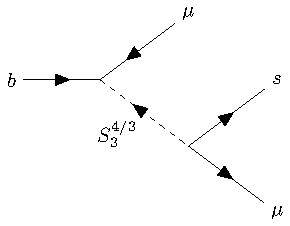
\includegraphics[width=0.4\linewidth]{ch4_bsmumu}
  \caption{The figure shows the diagram through which the $|Q| = 4/3$ component
    of $S_{3}$ mediates the $b \to s \mu\mu$ decays.}
  \label{fig:ch4-s3-bsmumu}
\end{figure}

As mentioned briefly above, the model is constructed so that $S_{3}$ can give
the dominant contribution to $C_{9} = -C_{10}$ [the direction characterised by
new physics in the operator $\mathcal{O}_{LL}$ of
Eq.~\eqref{eq:ch3-c9-c10-chiral}]. The $|Q| = 4/3$ component of the isotriplet
generates $\mathcal{O}_{LL}$ at tree-level, through the diagram shown in
Fig.~\ref{fig:ch4-s3-bsmumu}. As discussed in detail in
Chapter~\ref{chapter:the-one-lq}, $S_{1}$ contributes to the operators
$\mathcal{O}_{LL} \sim \mathcal{O}_{9} - \mathcal{O}_{10}$ and
$\mathcal{O}_{LR} \sim \mathcal{O}_{9} + \mathcal{O}_{10}$ at the loop level,
with the relevant expressions given by Eq.~\eqref{eq:ch3-cllclreqs}. We take
this contribution to be negligible, and concentrate on the tree-level generation
of the operator through $S_{3}$. Meeting the best-fit value
requires\footnote{Here and throughout this chapter, we use $C_{9,10}$ to
  represent the new-physics contribution to the muonic operator for brevity. We
  freely interchange between $C_{9,10}$ and $C_{9,10}^{\mu\mu}$, but we intend
  no difference between these.}
\begin{equation}
  \label{eq:ch4-c9c10}
  {C}_9= -{C}_{10} = - \frac{\pi \cos (\theta_L)}{2 \sqrt{2} G_F \alpha} \frac{1}{V_{tb}V_{ts}^*} \frac{x_{3}^{23} x_{3}^{22*}}{m_{S_{3}}^2} \approx -0.53 \ ,
\end{equation}
corresponding to the choice of couplings
\begin{equation}
 |x_{3}^{23} x^{22*}_{3} | \cos \theta_L \approx  \left(\frac{m_{S_{3}}}{\SI{24}{\TeV}} \right)^2 \ .
\end{equation}
Note that the couplings above are derived from a global fit to real valued
Wilson coefficients~\cite{Aebischer:2019mlg}. To ensure a ${C}_9=-{C}_{10}$
consistent with this, we fix the value of $C_9$ such that
$\text{Im}~C_9 \approx 0$. This requires a constraint to be imposed on the
Casas-Ibarra parametrisation, since Eq.~\eqref{eq:ch4-ci} in general generates
complex $x_{3}^{23}$, a point we elaborate on in
Sec.~\ref{sec:ch4-innes-results-and-disc}.

\subsubsection{Charged-current anomalies}

\begin{figure}[t]
  \centering
  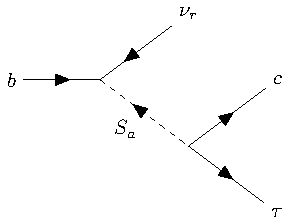
\includegraphics[width=0.4\linewidth]{ch4_bctaunu}
  \caption[The leading-order diagrams contributing to $R_{D}$ and $R_{D^{*}}$ in
  our model.]{The leading-order diagrams contributing to $R_{D}$ and $R_{D^{*}}$
    in our model. There are additional LNV diagrams that we ignore in our
    analysis.}
  \label{fig:ch4-bctaunu-diags}
\end{figure}

There are a number of contributions to $b \to c \tau \nu_{r}$ diagrams in our
model. Those which dominate are shown in Fig.~\ref{fig:ch4-bctaunu-diags}: the
ones mediated by the $|Q| = 1/3$ leptoquarks (of which one is present in the
$S_{3}$ multiplet). The additional diagrams involve only $S_{3}$ and are
lepton-number violating, and thus we expect them to be suppressed by the same
combination of parameters required to render the neutrino masses sufficiently
small. The diagrams in Fig.~\ref{fig:ch4-bctaunu-diags} imply the same set of
Wilson coefficients discussed in earlier chapters, see \textit{e.g.}
Eq.~\eqref{eq:ch3-ccoperators}. The neutrino flavour index $r$ is left general
since the process could be lepton-flavour violating, although only the vector
contribution with a tau neutrino (\textit{i.e.} $C_{V}$ with $r = 3$)
constructively interferes with the SM diagram. The contributions are
\begin{align}
[{C}_{S}]_{r} &= \frac{\sqrt{2}\cos \theta_L}{8 G_F V_{cb}} \left( \frac{x^{r3}_{1} y^{32*}_{1}}{m_{S_{1}}^2} \right) \ , \label{eq:ch4-csl} \\
[{C}_{V}]_{r} &= \frac{\sqrt{2}\cos \theta_{L}}{8 G_F V_{cb}} \left(\frac{x^{r3}_{1} z^{32*}_{1}}{m_{S_{1}}^2} - \frac{x_{3}^{r3} z_{3}^{32*}}{2 m_{S_{3}}^2} \right) \ , \label{eq:ch4-cvl} \\
[{C}_{T}]_{r} &=-\frac{1}{4} [C_{S}]_{r} \ . \label{eq:ch4-ct}
\end{align}
We will often use the notation that $C_{S,V,T}$, written without an explicit
index $r$, corresponds to $[C_{S,V,T}]_{3}$. In
Chapter~\ref{chapter:the-one-lq}, we saw that contributions to the vector
operator $C_{V}$ could only be mild on account of constraints from
$B \to K^{*}\nu\nu$ and $\bar{B}_{s}$--$B_{s}$ mixing. These constraints are
reassessed in this model to additionally acount for the role of $S_{3}$ in
Sec.~\ref{sec:ch4-innes-constraints}, although the simplest approach is to fit
$C_{S} = -4 C_{T}$ to the best-fit value of Table~\ref{tab:ch3-fitresults}:
$C_{S} = -4 C_{T} = 0.14$. This implies
\begin{equation}
  x_{1}^{33} y_{1}^{32*} \cos \theta_{L} \approx \left( \frac{m_{S_{1}}}{\SI{1.6}{\TeV}} \right)^{2} \ ,
\end{equation}
although contributions to the vector operator are inevitable for both
leptoquarks since $x_{1,3}^{33} \neq 0$, and $z^{32}$ is therefore necessarily
also non-zero on account of Eq.~\eqref{eq:ch4-z-relation}.


\subsubsection{Anomalous magnetic moment of the muon}

There are three diagrams contributing to the anomalous magnetic moment of the
muon in this model. These are known results, \textit{e.g.}~\cite{Bauer:2015knc,
  Dorsner:2016wpm}, and so we simply quote and interpret the results. The
contributions are
\begin{equation}
  \label{eq:ch4-amu-s1}
a_\mu^{S_{1}} = \sum_r \frac{m_\mu m_{u_r}}{4\pi^2 m_{S_{1}}^2} \left( \frac{7}{4} - \ln\frac{m_{S_{1}}^2}{m_{u_r}^2}\right) \text{Re} (y^{2r} z_{1}^{2r}) - \frac{m_\mu^2}{32\pi^2 m_{S_{1}}^2} \left(\sum_r |z^{2r}_{1}|^2+ \sum_r |y^{2i}|^2 \right) \ ,
\end{equation}
for $S_{1}$ [the same as Eq.~\eqref{eq:ch3-amu} with the analogous notation for
this model], and
\begin{equation}
a_\mu^{S_{3}} =  - \frac{m_\mu^2}{32\pi^2 m_{S_{3}}^2} \sum_r |z^{2r}_{3}|^2 \ ,
\end{equation}
for $S_{3}$. The same-chirality terms are suppressed by
$m_{\mu}^{2} / m_{S_{a}}^{2}$, and so negligibly small. This implies
non-vanishing right-handed couplings for the $S_{1}$ leptoquark. This is the
same situation as in Chapter~\ref{chapter:the-one-lq}, where it was found that
the scalar--tensor solution to $R_{D^{(*)}}$ could also accommodate the measured
value of $a_{\mu}$ easily, since $y^{23}$ is a free parameter unrelated to any
other anomalies and relatively unconstrained.

\subsection{Contraints}
\label{sec:ch4-innes-constraints}

Below we discuss the constraints relevant to our model and the limits we require
in our subsequent analysis. We restrict our main discussion to what we consider
to be the minimal scenario to explain the $B$ anomalies and $(g-2)_\mu$. Here,
the isotriplet leptoquark $S_{3}$ explains the neutral-current anomalies, while
the $\text{SU}(2)_{L}$ singlet $S_{1}$ explains the charged-current anomalies
with contributions to the scalar, tensor and vector operators. Minimally, this
implies non-zero values for $x_{1}^{33}$ and $y^{32}$. The top-mass enhancement
evident in Eq.~\eqref{eq:ch4-amu-s1} means that only small values for the
product of $y^{23}$ and $z_{1}^{23} = x_{1}^{23}$ are required to explain the
anomalous magnetic moment of the muon.

The $S_{3}$ leptoquark, which participates in the neutrino-mass generation, must
have a non-zero Yukawa coupling to the electron, and this is the most import
phenomenological consequence for the constraints we consider. This, together
with the relation in Eq.~\eqref{eq:ch4-z-relation}, means that constraints from
processes involving the first generation of SM fermions cannot be avoided
completely. In fact, the hierarchy present in the leptoquark couplings to
charged leptons is fixed by measured PMNS matrix elements, while the couplings
to light quarks are suppressed by CKM matrix elements. Explicitly
\begin{equation}
   \label{eq:ch4-yxckm}
  \begin{split}
    z_{3}^{rs} &= x_{3}^{r3} V_{s3}^* \\
    &= V_{s3}^* \frac{\zeta}{\sqrt{2m_0}} \left( \sqrt{m_2} u_{r2}^* + i \sqrt{m_3} u_{s3}^* \right) \ ,
  \end{split}
\end{equation}
where $m_{0} = m_{0}(3)$ of Eq.~\eqref{eq:ch4-ci-innes}. Of course, the
Lagrangian in Eq.~\eqref{eq:ch4-lag-y} contains many more parameters than these.
For simplicity, we turn off any couplings not immediately related to the
anomalies or neutrino mass. In reality these need only be small enough to
respect any limits placed on them by experiment\footnote{Note that constraints
  from neutrinoless double beta decay are not explicitly considered in this
  analysis. The contributions are CKM suppressed and the couplings involved are
  exactly those involved in the neutrino-mass generation. As such, new-physics
  contributions from this model to this process are negligible.}.

The constraints presented in this section assume the following set of non-zero
Yukawa couplings:
\begin{equation}
\mathbf{x}_{1} = \begin{pmatrix} 0 & 0 & 0 \\
                                0 & 0 & 0 \\
                                0 & 0 & x^{33}_{1}
                              \end{pmatrix}, \quad
\mathbf{y} = \begin{pmatrix} 0 & 0 & 0 \\
                             0 & 0 & y^{23} \\
                             0 & y^{32} & 0
                             \end{pmatrix}
                             \quad \text{ and } \quad
\mathbf{x}_{3} = \begin{pmatrix} 0 & 0 & x_{3}^{13} \\
                                 0 & x^{22}_{3} & x^{23}_{3} \\
                                 0 & 0 & x_{3}^{33}
                                \end{pmatrix} \ .
\end{equation}
It is understood that $w_{1}^r = 0$, since we work in the regime where $S_{1}$
does not contribute to the neutrino mass. We discuss other Yukawa-coupling
textures throughout this section where appropriate. Notably, we comment briefly
on explaining $R_{D^{(*)}}$ with contributions only to the vector operator
$C_{V}$, and the constraints associated with this scenario are presented in this
section as well.

This parameter space is explored in the context of the constraints implied by
fits to the flavour anomalies and neutrino mass. We use a suite of computational
machinery for most of the calculations, and this setup is discussed briefly
below. Where appropriate we explicitly write out the dominant contributions to
observables where we consider that this provides useful insight. Some
observables are also calculated separate to these methods, and these are also
discussed in detail below.

We use the computational frameworks \textsf{SARAH}~\cite{Porod:2014xia,
  Porod:2011nf} and \textsf{SPheno}~\cite{Porod:2011nf} to calculate Wilson
coefficients, decay rates and a subset of the flavour observables, defined by
\textsf{FlavorKit}~\cite{Porod:2014xia}, in our analysis. A full discussion of
the underlying machinery and relation between these programs can be found in
Ref.~\cite{Vicente:2015zba}. In addition, we use
\textsf{flavio}~\cite{Straub:2018kue} to calculate some flavour observables from
the Wilson-coefficient output files of \textsf{SPheno}. This allows us to
consider a broader range of flavour observables in our analysis. The
renormalisation-group running of Wilson coefficients in \textsf{flavio} is
implemented using the \textsf{Wilson} package~\cite{Aebischer:2018bkb}.

\subsubsection{Collider bounds}

The ATLAS collaboration has dedicated searches for the heavy quarks $B$ and $Y$.
The most stringent limits come from searches for singly produced $Y$ decaying to
$W b$, where a limit of $m_{Y} \gtrsim \SI{1.85}{\TeV}$ is set with 95\%
confidence~\cite{Aaboud:2018ifs}. Limits on the $B$ fermion come from searches
for singly produced $B$ decaying as $B \to Hb$~\cite{ATLAS-CONF-2018-024}, or
pair-produced $B$ decays through $B \to Zb/Hb/Wt$~\cite{Aaboud:2018pii}. The
latter search gives the more stringent limit of $m_{B} \gtrsim \SI{1.34}{\TeV}$.
In our phenomenological analysis, we take $m_{\chi}$ to be much larger than
these scales, safely avoiding the direct-production bounds.

Collider limits relevant for the scalar leptoquark $S_{1}$ are discussed in
Sec.~\ref{sec:ch3-thescalarleptoquarkmodel}. Here we extend the discussion to
$S_{3}$ as well. The $|Q| = 1/3$ component of $S_{3}$ contributes to the same
decay channels as $S_{1}$, that happen to be the most constraining. Thus, the
direct-production limits quoted in Sec.~\ref{sec:ch3-thescalarleptoquarkmodel}
apply also to the $S_{3}$ leptoquark.

In our model couplings of third-generation quarks to the muon through $S_{3}$
are unavoidable. Here, limits from $tt\mu\mu$ searches can exclude leptoquark
masses below \SI{1.3}{\TeV}, assuming
$\text{Br}(S_{a} \to t \mu) \approx 100\%$~\cite{Sirunyan:2018ruf}.
Additionally, since $S_{3}$ must couple the strange quark to the muon,
dimuon--dijet searches are also potentially relevant. In this case, the limits
can be as large as $m_{S_{3}} \gtrsim \SI{1.5}{TeV}$~\cite{Aaboud:2019jcc,
  Sirunyan:2018ryt}.

High-$p_T$ dilepton production through the $S_{3}$ leptoquark has also been
shown to provide interesting constraints and signatures for the leptoquarks in
our model~\cite{Angelescu:2018tyl}. The leptoquark contributes to the processes
$pp \to \ell \ell$ through tree-level $t$-channel graphs whose effects can alter
the tail of the differential cross-sections for $pp \to \ell \ell$. We take the
limits from Ref.~\cite{Angelescu:2018tyl} for the muon and tau modes derived
from \SI{36}{\per\fb} of ATLAS data at \SI{13}{\TeV}~\cite{Aaboud:2017sjh,
  Aaboud:2017buh}. We derive bounds on $bb \to ee$ and extract the
\SI{3000}{\per\fb} ATLAS sensitivity for the electron and muon modes from
Ref.~\cite{Greljo:2017vvb}. These bounds are shown in
Fig.~\ref{fig:ch4-lhcbounds}. We find that the limits on $cc \to ee$ and
$uu \to ee$ give less stringent bounds on $|\zeta|$, and thus we do not include
them in our numerical scans.

\begin{figure}[t]
  \centering
  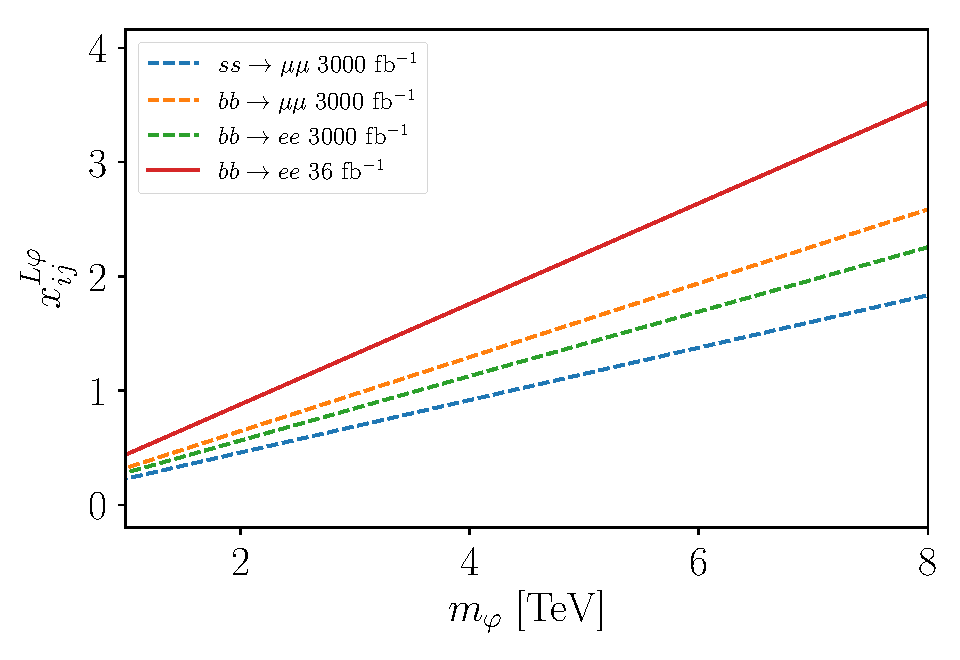
\includegraphics[width=0.7\textwidth]{lhcbounds.pdf}
  \caption[The figure shows the current (solid) and projected (dashed) upper
  limits on the couplings of the $S_{3}$ leptoquark to down-type quarks and
  charged leptons $x_{3}^{rs}$.]{The figure shows the current (solid) and
    projected (dashed) upper limits on the couplings of the $S_{3}$ leptoquark
    to down-type quarks and charged leptons $x_{3}^{rs}$. The limits are from
    LHC searches in $pp \to \ell \ell$ high-$p_T$ tails at \SI{13}{\TeV} from
    ATLAS~\cite{ATLAS-CONF-2017-027}, derived from Ref.~\cite{Greljo:2017vvb}.
    The Yukawa coupling being constrained depends on the process. For example,
    $ss \to \mu \mu$ will constrain $x^{22}_{3}$.}
  \label{fig:ch4-lhcbounds}
\end{figure}


\subsubsection{Fermion mixing}

Of central importance in this model is the mixing generated by the terms
$x^{3}_{d} \bar{b}_R H \chi_L + \text{h.c.}$ between the $b$ quark and the quark
field $\chi_{L}$. This mixing is a necessary ingredient for the violation of
lepton number by $S_{3}$, and plays a governing role in the overall scale of the
neutrino mass $m_0 = m_{0}(3)$ according to Eq.~\eqref{eq:ch4-ci}. Its size also
dictates the extent to which $\Delta L=2$ neutrino final states are important to
consider, for example in $B \to K^{(*)} \nu \nu$.

The mixing of the $b$ with $\chi$ leads to new contributions to the oblique
electroweak parameters $S$ and $T$. These have been measured to high precision
by LEP~\cite{ALEPH:2005ab}. The mixing also leads to an alteration of the $Zbb$
coupling at tree-level, for which global electroweak fits have suggested a small
deviation from the SM value, \textit{e.g.}~\cite{Ciuchini:2013pca}. The dominant
contributions to these effects are encapsulated in the effective dimension-six
Lagrangian generated by the heavy $\chi_{L} + \chi_{R}$ at the scales probed by
experiment:
\begin{equation}
\mathcal{L}^{(6)}_{\chi} \supset \frac{C^{33}_{Hd}}{m_\chi^2} (H^\dagger i \overset{\leftrightarrow}{D}_\mu H) (\bar{b}_R \gamma^\mu b_R) + \frac{C^{33}_{dH}}{m_\chi^2} y_b (H^\dagger H) (\bar{Q}_3 b_R H).
\end{equation}
The first operator modifies the electroweak precision observables discussed
above and the second affects Higgs measurements and is currently poorly
constrained. We take the $2\sigma$ bounds on the operator coefficient
$C_{Hd}^{33}$ from the electroweak fit performed in Ref.~\cite{Ciuchini:2013pca}
$C_{Hd}^{33} \in [-0.38, 0.03]$ to derive
\begin{equation}
    \label{eq:ch4-bmixinglimit}
    |x_{d}^{3}| \in [0.25, 0.87] \left( \frac{m_\chi}{\TeV} \right).
\end{equation}
This implies the bounds $\theta_R \in [0.06, 0.21]$ at $95\%$ confidence, with
central value $\theta_R \approx 0.16$. This agrees with
Ref.~\cite{Aguilar-Saavedra:2013qpa} which studied the effects of the doublets
$\chi_{L} + \chi_{R}$ and other vector-like quarks. The relation
$\theta_L \approx \frac{m_b}{m_\chi} \theta_R$ from Eq.~\eqref{eq:ch4-bmixing}
implies the $\cos \theta_L$ factors appearing in Eq.~\eqref{eq:ch4-c9c10} and
Eq.~\eqref{eq:ch4-csl}--\eqref{eq:ch4-ct} do not suppress the contributions to
the anomalous observables\footnote{This result is a stronger, and more general,
  constraint than that quoted from direct searches in
  Ref.~\cite{Aaboud:2018ifs}, which suggests a $95\%$ confidence interval of
  $\sin \theta_R \in [0.17,0.55]$ for $m_\chi \sim \SI{800}{\GeV}$.}.
Restricting this mixing to be small consequentially reduces the mass-splitting
between the components of the exotic doublets $\chi_{L} + \chi_{R}$, such that
$m_{\chi} \sim m_{B} \sim m_{Y}$ remains a valid approximation.

\subsubsection{Lepton-flavour violation}

Both leptoquarks contribute to lepton-flavour violating processes, although the
diagrams involving both the left- and right-handed Yukawa couplings of $S_{1}$
are generally dominant due to the top-enhancement in expressions, see
\textit{e.g.} Ref.~\cite{Angel:2013hla}. In our analysis we calculate LFV
observables using the \textsf{SARAH} and \textsf{SPheno} pipeline discussed
above. We present a summary of the processes we include in our phenomenological
analysis along with the limits we impose in Table~\ref{tab:ch4-lfv-summary}.

\begin{table}[t]
  \centering
  \bgroup
  \def\arraystretch{1.3}
  \begin{tabular}{cc}
    \toprule
    Process & Limit \\
    \midrule
    $\text{Br}(\mu \to e \gamma)$ & $< 4.2 \cdot 10^{-13}$   \\
    $\text{Br}(\mu \to 3 e)$ &  $< 1.0 \cdot 10^{-12}$  \\
    $\frac{\sigma(\mu \text{Au}\to e\text{Au})}{\sigma(\mu \text{Au}\to \text{capture})}$ &  $< 7.0 \cdot 10^{-13}$  \\
    $\text{Br}(\tau \to e \gamma)$ & $< 3.3 \cdot 10^{-8}$   \\
    $\text{Br}(\tau \to \mu \gamma)$ &$< 4.4 \cdot 10^{-8}$    \\
    $\text{Br}(\tau \to 3\mu)$ &  $< 2.1 \cdot 10^{-8}$  \\
    $\text{Br}(\tau \to 3 e)$ &  $< 2.7 \cdot 10^{-8}$  \\
    \bottomrule
  \end{tabular}
  \egroup
  \caption[The table shows the limits we take on the LFV processes considered in
  our analysis~\cite{PhysRevD.98.030001}.]{The table shows the limits we take on
    the LFV processes considered in our analysis~\cite{PhysRevD.98.030001}.
    These are calculated using \textsf{SARAH} and \textsf{SPheno}.}
  \label{tab:ch4-lfv-summary}
\end{table}

\subsubsection{$Z$ decays}

The leptoquarks $S_{1}$ and $S_{3}$ will modify the $Z$ coupling to leptons
through one-loop diagrams involving SM quarks and the vector-like quark
$\chi_{L} + \chi_{R}$. For the contributions involving leptoquarks and SM
fermions we use the results of Ref.~\cite{Arnan:2019olv}, which include
corrections due to the external momenta of the $Z$. The additional diagrams with
the vector-like quark in the loop are shown in Fig.~\ref{fig:ch4-Zchidiags}. We
find the contributions to the leptonic $Z$ couplings from these to be
\begin{align}
    \delta g_{L}^{r s} &= \frac{w_{3}^{s} w_{3}^{r*}}{768 \pi^2 x (x - 1)^4} [x_Z f(x) + x_Z^2 g(x)]
\end{align}
where $x \equiv m_\chi^2 / m_{S_{3}}^2$, $x_Z \equiv m_Z^2 / m_{S_{3}}^2$ and
the functions $f(x)$ and $g(x)$ are
\begin{align}
  \begin{split}
    f(x) &= 3 x (x - 1) \left[ (4x^3 - 30x + 20) - (x - 1) (19x^2 - 53x + 28) \log x \right]\\ &\quad + 6x\cos^2 \theta_W(x-1) \left[ (x-1)(x^2 - 17x + 10) + 2(x^3 + 6x - 4) \log x \right]
  \end{split} \\
  \begin{split}
    g(x) &= 5(x-1)(x^3 - 5x^2 + 13x + 3) + 60 x \log x\\ &\quad + \cos^2\theta_W \left[4(x-1)(x^3 - 5x^2 + 13x + 3) - 48 x \log x  \right].
  \end{split}
\end{align}
The couplings $w_{3}^{r}$ are inversely proportional to $\zeta$, and thus we
expect these contributions to be suppressed when $\zeta$ and the $\chi$--$b$
mixing parameter $x_{d}^{3}$ are sizeable.

\begin{figure}[t]
  \centering
  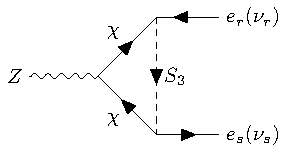
\includegraphics[width=0.45\textwidth]{z_chi_diag_1}
  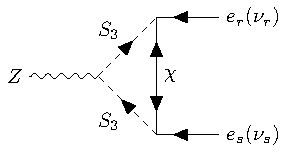
\includegraphics[width=0.45\textwidth]{z_chi_diag_2}
  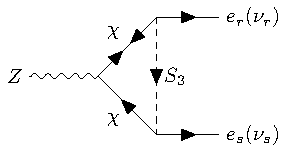
\includegraphics[width=0.45\textwidth]{z_chi_diag_3}
  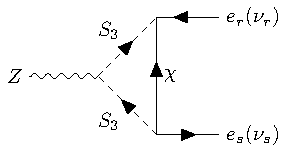
\includegraphics[width=0.45\textwidth]{z_chi_diag_4}
  \caption[The figure shows the additional diagrams contributing to
  $Z \to e_{r} e_{s}$ and $Z \to \nu_{r} \nu_{s}$ involving both $\chi$ and
  $S_{3}$ in our model.]{The figure shows the additional diagrams contributing
    to $Z \to e_{r} e_{s}$ and $Z \to \nu_{r} \nu_{s}$ involving both $\chi$ and
    $S_{3}$ in our model. In all cases, there are diagrams with $B$ and $Y$ in
    the loop with different charge states of $S_{3}$.}
  \label{fig:ch4-Zchidiags}
\end{figure}

\subsubsection{Charm-meson decays}

Since couplings to up-type quarks and charged leptons cannot be avoided for the
leptoquark that couples to $\chi$, the physics of operators of the form
$O_{rstu} \sim (u_r \Gamma u_s)(\ell_t \Gamma \ell_u)$ is important to study.
Here, we consider the leptonic decays of the $D^0$ meson, since a sizeable
coupling to the charm quark can assist in the explanation of the large effects
seen in the charged current anomalies~\cite{Fajfer:2015mia}.

In Sec.~\ref{sec:ch3-constraints} we saw that $S_{1}$ generates the entire
spectrum of operators which can in principle contribute to the leptonic decays
of the $D^0$, since it interacts with both left- and right-chiral SM fermions.
Concretely, the dimension-six Lagrangian of Eq.~\eqref{eq:ch3-charm-lag},
repeated here in a slightly altered notation:
\begin{equation}
  \begin{split}
    \mathcal{L}_{u_r u_s e_t e_u}
    &= \frac{4 G_F}{\sqrt{2}} \bigg[  C^{rstu}_{D,V_{R}}  (\bar{u}_r \gamma_\mu P_R u_s)(\bar{e}_t \gamma^\mu P_R e_u) + C_{D,V_{L}}^{rstu} (\bar{u}_r \gamma_\mu P_L u_s)(\bar{e}_t \gamma^\mu P_L e_u)\\ &\quad + C_{D,T}^{rstu} (\bar{u}_r \sigma_{\mu\nu} P_R u_s)(\bar{e}_t \sigma^{\mu\nu} P_R e_u) + C_{D,S_L}^{rstu} (\bar{u}_r P_L u_s)(\bar{e}_t P_L e_u)\\ &\quad + C_{D,S_R}^{rstu}(\bar{u}_r P_R u_s)(\bar{e}_t P_R e_u) + \text{h.c.}
    \bigg] \ ,
  \end{split}
\end{equation}
is generated with tree-level contributions from both leptoquarks:

\begin{align}
  C_{D,V_L}^{rstu} &= \frac{1}{2\sqrt{2} G_F} \left(\frac{z^{ts}_{1} z^{ur*}_{1}}{2m_{S_{1}}^2} + \frac{z_{3}^{ts} z_{3}^{ur*}}{m_{S_{3}}^2} \right) \ , \\
  C_{D,V_R}^{rstu} &= \frac{1}{4\sqrt{2} G_F} \frac{y^{ts*} y^{ur}}{m_{S_{1}}^2} \ , \\
  C_{D,S_L}^{rstu} &= \frac{1}{4\sqrt{2} G_F} \frac{z_{1}^{ts}y^{ur}}{m_{S_{1}}^2} \ , \\
  C_{D,S_R}^{rstu} &= \frac{1}{4\sqrt{2} G_F} \frac{y^{ts*} z^{ur*}_{1}}{m_{S_{1}}^2} \ , \\
  C_{D,T}^{rstu} &= -\frac{1}{4} C^{rstu}_{D,S_L} \ ,
\end{align}

\noindent although in our phenomenological analysis only the relevant $S_{3}$ couplings
are present.

As highlighted in Ref.~\cite{Fajfer:2015mia}, the strongest experimental
constraints on these coefficients come from measurements of the process
$D^0 \to \mu\mu$, for which Eq.~\eqref{eq:ch3-Dmumu} is relevant. We impose the
experimental upper limit
$\text{Br}(D^0 \rightarrow \mu\mu) < 7.6 \cdot 10^{-9}$~\cite{Aaij:2013cza}.
Contributions to the electronic mode from the vector operators are helicity
suppressed and we ensure $|y^{1r}| \ll 1$ in all numerical scans to avoid
contributions to the electronic scalar and tensor operators.


\subsubsection{Bottom-meson decays and mixing}

Here we consider the decays $B \to K^{(*)} \nu\nu$ and constraints from
$\bar{B}_{s}$--$B_{s}$ mixing, found to be very important constraints on the BN
scenario for explaining $R_{D}$ and $R_{D^{*}}$.

We saw in Sec.~\ref{sec:ch3-raremesondecays} that $S_{1}$ contributed to the
decays $B \to K^{(*)} \nu \nu$ through contributions to a vector four-fermion
operator. There are similar contributions to the same operator
\begin{equation}
  \label{eq:onunu}
  \mathcal{O}^{rs}_{\nu\nu} =\frac{8 G_F}{\sqrt{2}} \frac{\alpha}{4\pi} V_{tb} V_{ts}^*[\bar{\nu}_r  \gamma_\mu P_L \nu_s][\bar{s} \gamma^\mu P_L b] \ ,
\end{equation}
also from $S_{3}$ in this case. That is:
\begin{equation}
  C_{\nu\nu}^{rs} = \frac{\cos \theta_L}{2\sqrt{2} G_F V_{tb} V_{ts}^*} \frac{4\pi}{\alpha} \left( \frac{x_{1}^{r3} x^{s2*}_{1}}{m_{S_{1}}^2} + \frac{x^{r3}_3   x^{s2*}_{3} }{2m_{S_{3}}^2}\right) \ .
\end{equation}
The presence of both contributions presents the possibility of arranging for a
cancellation. This approach has been employed in the literature to recover an
explanation of $b \to c$ data with only contributions to the vector
operator~\cite{Crivellin:2017zlb}. We impose $R_{K^{*}}^{\nu\nu} < 2.7$, as in
Sec.~\ref{sec:ch3-raremesondecays}, in our numerical analysis.

The process of $B_s$--$\bar{B}_s$ mixing provides a complementary constraint on
the same couplings involved in the $b \to s \nu \nu$ processes. It was found in
Chapter~\ref{chapter:the-one-lq} that the process leads to a weaker constraint
than $B \to K \nu \nu$ and $B \to K^* \nu \nu$ for low $S_{1}$ masses, but
becomes relevant for masses larger than a few \TeV. In our model, we have
contributions from both the isosinglet and isotriplet leptoquarks through box
diagrams with neutrinos and charged leptons in the loop. These contribute to the
operator $C^{bs}_1$,
\begin{equation}
\mathcal{L}_{\Delta B = 2} \supset  C^{bs}_1 (\bar{b} \gamma_\mu P_L s)(\bar{b} \gamma^\mu P_L s),
\end{equation}
where colour indices are contracted within parentheses. The combination
$C_{B_s} \exp{2 i \phi_{B_s}} = \Delta m_s^{\text{exp}} / \Delta m_s^{\text{SM}}$
is calculated using \texttt{SPheno}~\cite{Vicente:2015zba, Porod:2003um,
  Porod:2011nf}, and we impose the UT\textit{fit} collaboration's
result~\cite{Bona:2007vi}
\begin{equation}
C_{B_s} = 1.110 \pm 0.090
\end{equation}
in our numerical scans. We will work with small imaginary parts for the
couplings fixed by the neutrino mass and we maintain $\phi_{B_s} \approx 0$ for
the phase, consistent with UT\textit{fit}'s result.

\subsubsection{Summary of constraints}

In Tables~\ref{tab:ch4-lfv-summary} and \ref{tab:ch4-summary} we present
summaries of the constraints of this section. The tables contain the observables
we consider in our later phenomenological analysis as well as the limits we
require.

\begin{table}
  \centering
  \begin{tabular}{ccc}
    \toprule
    Process & Quantity & Requirement \\
    \midrule
    $ss \to \mu \mu$                 &  $|x^{22}_{3}|$ & $< 0.41 m_{S_3} / \TeV$~\cite{Angelescu:2018tyl} \\
    $bb \to \mu \mu$                 &  $|x^{23}_{3}|$ & $< 0.58 m_{S_3} / \TeV$~\cite{Angelescu:2018tyl} \\
    $ss \to \tau \tau$                 &  $|x^{32}_{3}|$ & $< 0.54 m_{S_3} / \TeV$~\cite{Angelescu:2018tyl} \\
    $bb \to \tau \tau$                 &  $|x^{33}_{3}|$ & $< 0.80 m_{S_3} /  \TeV$~\cite{Angelescu:2018tyl} \\
    $bb \to e e$                 &  $|x^{13}_{3}|$ & $< 0.44 m_{S_3} / \TeV$~\cite{Greljo:2017vvb} \\
    $Z \to b b$                      &  $C_{Hd}^{33}$ & $\in [-0.38, 0.03]$~\cite{Ciuchini:2013pca} \\
    $\tau \to \eta e$                &  Br  & $< 9.2 \cdot 10^{-8}$ \\
    $\tau \to \pi e$                 &  Br  & $< 8.0 \cdot 10^{-8}$ \\
    $\tau \to \phi \mu$              &  Br  & $< 8.4 \cdot 10^{-8}$ \\
    $Z \to e^{\pm} \mu^{\mp}$                    &  Br  & $< 7.5 \cdot 10^{-7}$ \\
    $Z \to e^{\pm} \tau^{\mp}$                   &  Br  & $< 9.8 \cdot 10^{-6}$ \\
    $Z \to \mu^{\pm} \tau^{\mp}$                 &  Br  & $< 1.2 \cdot 10^{-5}$ \\
    $Z \to e_r e_s$                      &  $g_{L}$  & $\in [-8.5, 12] \cdot 10^{-4}$ \\
    $Z \to e_r e_s$                      &  $g_{R}$  & $\in [-5.4, 6.7] \cdot 10^{-4}$ \\
    $Z \to \nu_r \nu_s$              &  $N_\nu$  & within $2.9840 \pm 0.0164$ \\
    $D^0 \to \mu \mu$                &  Br  & $< 7.6 \cdot 10^{-9}$~\cite{Aaij:2013cza} \\
    $B^+ \to K^+ e^{\pm} \mu^{\mp}$                  &  Br  & $< 9.1 \cdot 10^{-8}$ \\
    $B^0 \to K^{0*} e^{\pm} \mu^{\mp}$                &  Br  & $< 1.8 \cdot 10^{-7}$ \\
    $B_s \to \mu^{\pm} e^{\mp}$                  &  Br  & $< 5.4 \cdot 10^{-9}$ \\
    $B \to D \ell \nu$               &  $R_{D}^{\mu / e} = \frac{\text{Br}(B \to D \mu \nu)}{\text{Br}(B \to D e \nu)}$  & within $0.995 \pm 0.090$~\cite{Glattauer:2015teq} \\
    $B \to D^* \ell \nu$             &  $R_{D^*}^{e / \mu} = \frac{\text{Br}(B \to D^* e \nu)}{\text{Br}(B \to D^* \mu \nu)}$  & within $1.04 \pm 0.10$~\cite{Abdesselam:2017kjf} \\
    $B_s$--$\bar{B}_s$ mixing        &  $C_{B_s}$  & $\in [0.942, 1.288]$~\cite{Bona:2007vi} \\
    $B \to K \nu \nu$                 &  $r_K^{\nu\nu} = \frac{\text{Br}}{\text{Br}_{\text{SM}}}$ & $< 3.9$~\cite{Grygier:2017tzo} \\
    $B \to K^* \nu \nu$                 &  $r_{K^*}^{\nu\nu} = \frac{\text{Br}}{\text{Br}_{\text{SM}}}$ & $< 2.7$~\cite{Grygier:2017tzo}\\
    $b \to s \gamma$                 &  Br & $\in [-0.17, 0.24]$~\cite{Amhis:2014hma} \\
    $B_c \to \tau \nu$                 &  Br & $< 30 \%$~\cite{Alonso:2016oyd} \\
    $K \to \ell \nu$                 &  $r_K^{\mu/e} = \frac{\text{Br}(K \to e \nu)}{\text{Br}(K \to \mu \nu)}$  & within $(2.488 \pm 0.018) \cdot 10^{-5}$\\
    \bottomrule
  \end{tabular}
  \caption[The table is a summary of the constraints considered in this section,
  not also mentioned in Table~\ref{tab:ch4-lfv-summary}.]{The table is a summary
    of the constraints considered in this section, not also mentioned in
    Table~\ref{tab:ch4-lfv-summary}. In cases where opposite-sign lepton pairs
    can have differing flavour, we choose the observable with both combinations
    of signs averaged. For the rare tau decays not elsewhere referenced, we have
    included only those which we found gave most competitive constraints. Where
    citations are omitted the requirements are taken from
    Ref.~\cite{PhysRevD.98.030001}.}
  \label{tab:ch4-summary}
\end{table}

\subsection{Results and discussion}
\label{sec:ch4-innes-results-and-disc}

Below we explore the extent to which this model can accommodate the charged- and
neutral-current anomalies, the anomalous magnetic moment of the muon and
neutrino mass in light of the constraints presented in the previous section.

First, we review the minimal setup introduced at the beginning of
Section~\ref{sec:ch4-innes-constraints} and present the results of our Monte
Carlo analysis. We also comment briefly on non-minimal scenarios.

\subsubsection{Monte Carlo analysis}

In the minimal scenario the deviations in $R_{D^{(*)}}$ are explained by the
isosinglet leptoquark $S_{1}$ with contributions in the direction
$C_{S_L}(m_{S_{1}}) = -4 C_T(m_{S_{1}})$, implying $\mathcal{O}(1)$ values for
the couplings $x_{1}^{33}$ and $y^{32}$~\cite{Cai:2017wry, Angelescu:2018tyl,
  Feruglio:2018fxo}. Contributions to the vector operator are more heavily
constrained since they necessarily imply large effects in $B \to K^{(*)} \nu\nu$
and $B_s$--$\bar{B}_s$ mixing, in the absence of any kind of cancellation. The
$S_{1}$ particle also explains the anomalous magnetic moment of the muon with
the values of $y^{23}$ and $z_{1}^{23} = x_{1}^{23}$ fixed according to
Eq.~\eqref{eq:ch4-amu-s1}. The limits derived in Ref.~\cite{Bigaran:2019bqv} and
sketched out in Sec.~\ref{sec:ch4-innes-neutrino-mass} suggest the extent to
which $S_{1}$ can contribute to the generation of neutrino masses is small.
Since we consider suppressed leptoquark mixing, this means there is no
connection between the neutrino-mass mechanism and the anomalies in
$R_{D^{(*)}}$ and $(g-2)_{\mu}$ in this model. For this reason, we fix
$m_{S_{1}}$ and the couplings involved in Eq.~\eqref{eq:ch4-amu-s1} and
Eq.~\eqref{eq:ch4-csl} to meet the respective central values to explain these
deviations. Explicitly, the conditions
\begin{equation}
\text{Re}(x_{1}^{23} y^{23}) \approx \frac{0.004 \hat{m}_{S_{1}}^2}{1 + \log \hat{m}_{S_{1}}} \quad \text{ and } \quad x_{1}^{33} y^{32} \approx 2.7 C_{S} \hat{m}_{S_{1}}^2,
\end{equation}
[with $\hat{m}_{S_{1}}$ defined as in Eq.~\eqref{eq:ch3-m-hat}] are met with
$m_{S_{1}} = \SI{2}{\TeV}$, $C_{S} = 0.14$, $x^{33}_{3} = 0.7$, $y^{32} = 2.15$,
$y^{23} = 0.5$ and $x^{23}_{1} = 0.02$ in all results presented in this section.
Many of the implications of explaining $R_{D^{(*)}}$ with
$C_{S_L} (\Lambda) = -4 C_T(\Lambda)$ have been discussed in the
literature~\cite{Feruglio:2018fxo, Asadi:2018sym, Alok:2019uqc}, and we have
expanded on this in Sec.~\ref{sec:ch3-resultsanddiscussion}.

The isotriplet scalar $S_{3}$ explains the neutral-current anomalies and
participates in the neutrino-mass generation. Thus, the couplings entering the
expression for $C^{\mu\mu}_{9} = - C^{\mu\mu}_{10}$ [Eq.~\eqref{eq:ch4-c9c10}]
are fixed by the Casas--Ibarra parametrisation, itself following from the
structure of the neutrino-mass matrix. A consequence of this is that the
$x^{r3}_{3}$ take complex values and in general
$\text{Im}(C^{\mu\mu}_{9}) \neq 0$. Indeed, for $\zeta \in \mathbb{R}$ the
imaginary part of $C^{\mu\mu}_{9}$ is much larger than the real part, since
$\text{Re}(x^{23}_{3}) = \sqrt{m_{2}/m_{3}} \text{Im}(x^{23}_{3})$ from
Eq.~\eqref{eq:ch4-ci-innes}. Although
$\text{Im} C^{\mu\mu}_{9} > \text{Re} C^{\mu\mu}_{9}$ may lead to an acceptable
explanation of the $b \to s$ anomalies (see \textit{e.g.} Appendix C of
Ref.~\cite{Altmannshofer:2014rta}), most fits in the literature assume
$\text{Im} C^{\mu\mu}_{9} = 0$ and we aim to reproduce this in our model as
well. The simplest way to do this is to assume $\arg \zeta \approx \pi / 2$, so
that $\zeta$ is mostly imaginary. This now implies
$\text{Re}(x^{23}_{3}) = \sqrt{m_{3}/m_{2}} \text{Im}(x^{23}_{3})$, and so the
muonic couplings of $S_{3}$ are mostly real.

One may worry that the central value of $\delta_{CP}$ (used in our numerical
analysis) or a non-zero value for the Majorana phase $\alpha_{2}$ will spoil the
desired $\text{Im} C^{\mu\mu}_{9} \ll \text{Re} C^{\mu\mu}_{9}$. Using
$\text{Im}C^{\mu\mu}_{9} / \text{Re}C^{\mu\mu}_{9} = \tan \arg C_{9}^{\mu\mu}$ as a
measure of the relative size of imaginary part of $C_{9}^{\mu\mu}$, we find
\begin{equation}
  \label{eq:ch4-c9rat}
  \begin{split}
    \tan \arg C_{9}^{\mu\mu} &\approx - \cot \arg \zeta\\
    &\quad + \sqrt{\frac{m_{2}}{m_{3}}}[0.085 \cos (\alpha_{2} + \delta_{CP}) - 0.72 \cos\alpha_{2}] \csc^{2}\arg \zeta+ \mathcal{O}\left(\frac{m_{2}}{m_{3}}\right) \ ,
  \end{split}
\end{equation}
for our model, derived from Eq.~\eqref{eq:ch4-ci-innes} and
Eq.~\eqref{eq:ch4-c9c10}. This clarifies that the effects of the phases are
subleading in $\sqrt{m_{2} / m_{3}}$. In figure~\ref{fig:ch4-c9rat} we plot
$\text{Im}(x_{3}^{r3}) / \text{Re}(x_{3}^{r3})$ for $r = 1, 2, 3$ as contours
with varying $\arg \zeta$ and $\alpha_{2}$. This illustrates the behaviour
discussed above but also investigates the effect on the other leptonic
couplings. It is evident that the choice $\arg \zeta \approx \pi/2$ also leaves
the tau coupling mostly real, although this cannot be said for the electron
coupling where the dependence on $\alpha_{2}$ is significant. We nevertheless
proceed with the choice $\arg \zeta = \pi / 2$ in our numerical analysis and
account for the possibility of a large imaginary part in the coupling
$x^{13}_{3}$.

\begin{figure}[t]
  \centering
  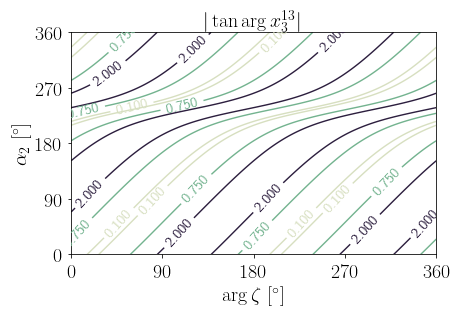
\includegraphics[width=0.49\textwidth]{c9rate}
  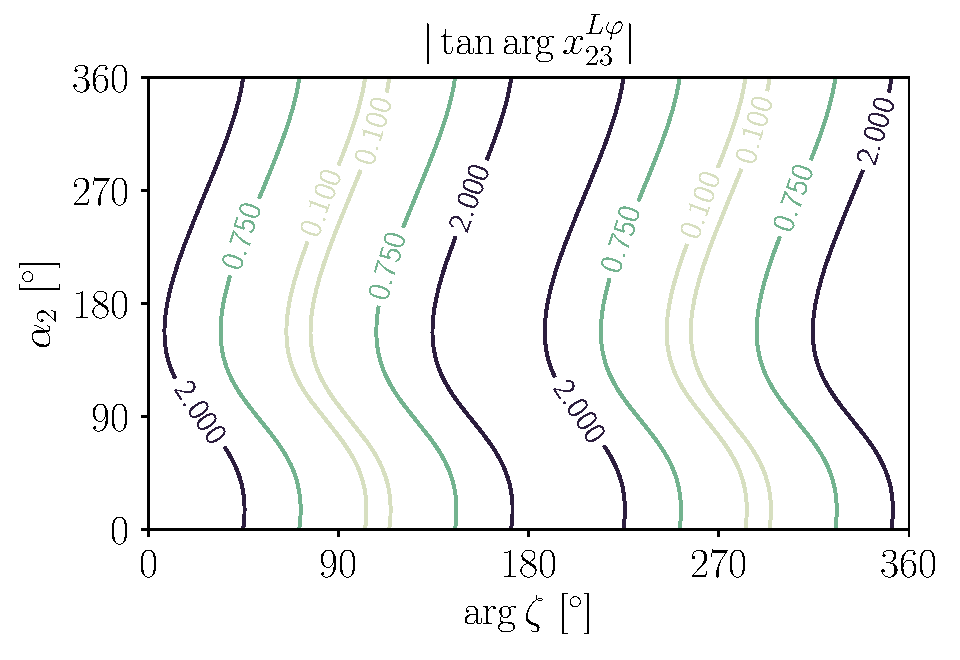
\includegraphics[width=0.49\textwidth]{c9ratmu}
  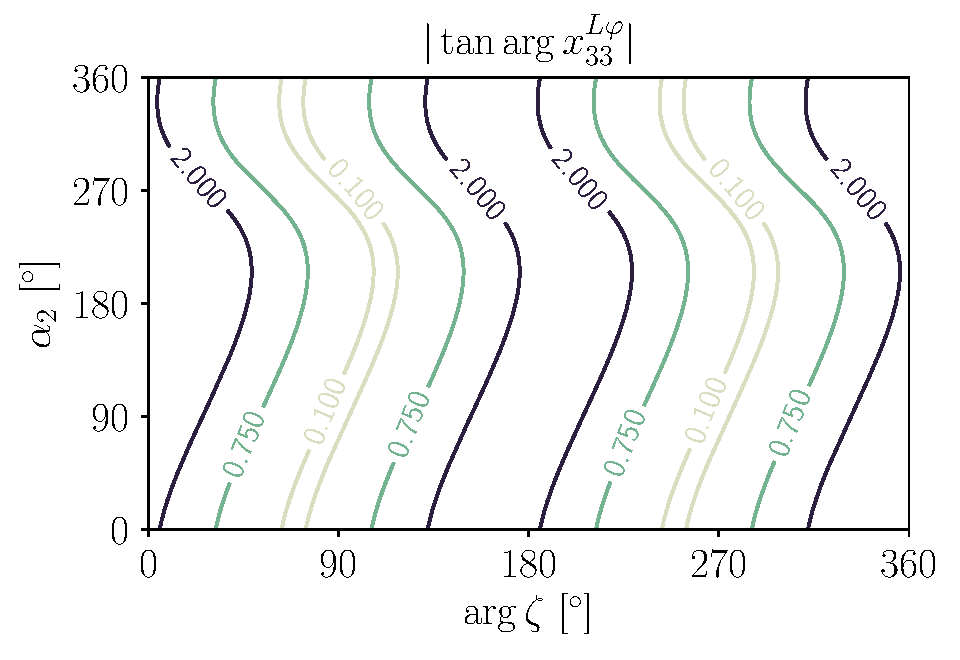
\includegraphics[width=0.49\textwidth]{c9rattau}
  \caption[Contours of
    $|\tan \arg x^{r3}_{3}| = |\text{Im}(x_{3}^{r3}) / \text{Re}(x_{3}^{r3})|$
    with varying $\arg \zeta$ and Majorana phase $\alpha_{2}$.]{Contours of
    $|\tan \arg x^{r3}_{3}| = |\text{Im}(x_{3}^{r3}) / \text{Re}(x_{3}^{r3})|$
    with varying $\arg \zeta$ and Majorana phase $\alpha_{2}$. The index $r$
    enumerates over charged-lepton flavours. It is clear that the choice
    $\arg \zeta \approx \pi/2$ ensures
    $\text{Im}x_{3}^{r3} \ll \text{Re}x_{3}^{r3}$ for the muon and tau couplings
    ($r = 2, 3$). The ratio of the imaginary and real parts of the electron
    coupling ($r = 1$) varies significantly with $\alpha_{2}$. The Dirac phase
    and all other neutrino parameters have been set to their central values.}
  \label{fig:ch4-c9rat}
\end{figure}

To explore the extent to which this scenario can explain the flavour anomalies
and neutrino mass, we perform a random scan over the 5 free parameters of the
setup: $|\zeta|$, $x_{3}^{22}$, $m_{S_{3}}$, $m_{\chi}$, $\alpha_{2}$. Random
values are drawn uniformly over the intervals defined for these parameters in
Table~\ref{tab:ch4-scenarioi}. Notably, the Yukawa coupling $x_{d}^{3}$ is fixed
to $0.25 m_{\chi} / \TeV$, the lower edge of the $2\sigma$ region from
Eq.~\eqref{eq:ch4-bmixinglimit} needed to explain the small discrepancy in
$Z \to b\bar{b}$. We generate $2 \cdot 10^6$ points which are filtered through
all of the constraints presented in section.~\ref{sec:ch4-innes-constraints}.

\begin{table}[t]
  \centering
  \begin{tabular}{l|ccccc}
    \toprule
    Parameters & $|\zeta|$ & $x_{3}^{22}$ & $m_{S_{3}}$ & $m_{\chi}$ & $\alpha_{2}$ \\
    \midrule
    Interval & $[1, 600]$ & $[0, \sqrt{4\pi}]$ & $[1, 30] \text{ TeV}$ & $[1, 10] \text{ TeV}$ & $[0, 2\pi]$ \\
    \bottomrule
  \end{tabular}
  \caption[The table shows the intervals from which the corresponding free
  parameters are randomly drawn for our Monte Carlo analysis.]{The table shows
    the intervals from which the corresponding free parameters are randomly
    drawn for our Monte Carlo analysis. All other parameters are fixed, see the
    text for details.}
  \label{tab:ch4-scenarioi}
\end{table}

 \begin{figure}[t]
  \centering
  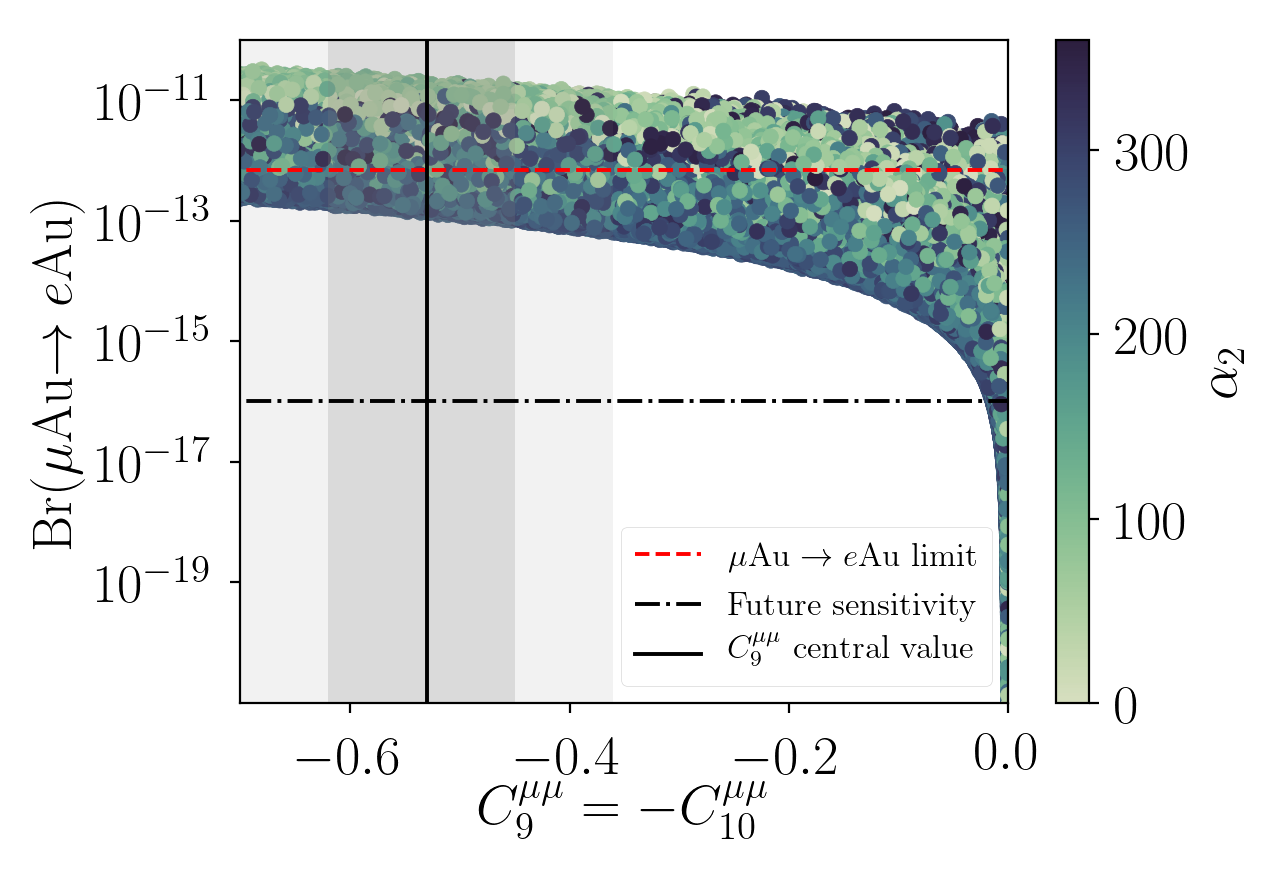
\includegraphics[width=0.495\linewidth]{m2ecVSc9.png}
  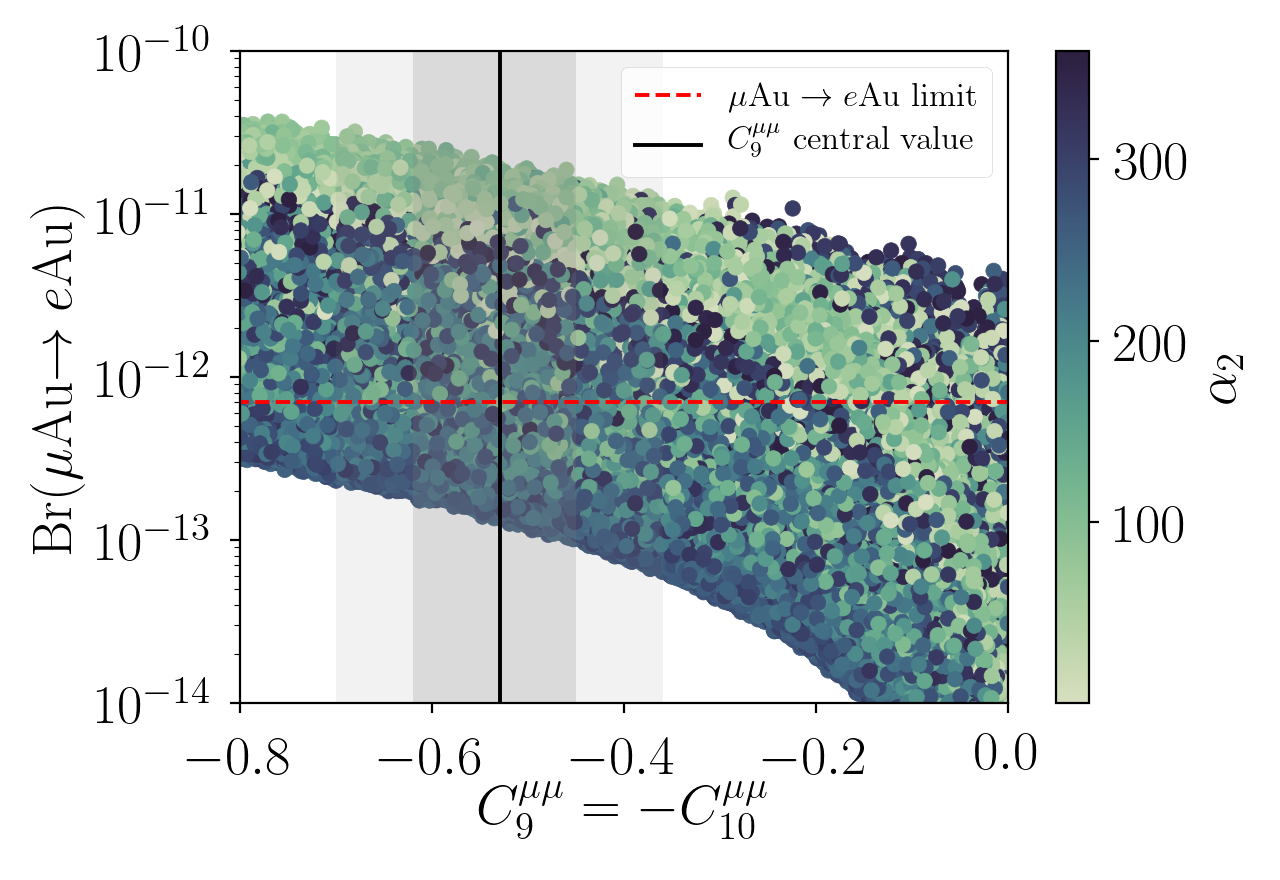
\includegraphics[width=0.495\linewidth]{m2ecVSc9Zoom.png}
  \caption[The results of the random scan projected onto
  $\text{Br}(\mu \text{Au} \to e \text{Au})$ and $C_{9}^{\mu\mu}$.]{The results
    of the random scan projected onto $\text{Br}(\mu \text{Au} \to e \text{Au})$
    and $C_{9}^{\mu\mu}$. All constraints except muon--electron conversion in
    Gold have been applied. The solid black line represents the central value of
    the fit of Ref.~\cite{Aebischer:2019mlg} to the anomalous $b \to s$ data,
    and the heavier and lighter shaded regions are the $1$ and $2\sigma$
    regions. The dashed red line corresponds to the current most stringent limit
    on $\text{Br}(\mu \text{Au} \to e \text{Au})$ from SINDRUM
    II~\cite{Bertl:2006up} and the black dot-dashed line is a representation of
    the projected sensitivity of future experimental reach \cite{KURUP201138,
      Cui:2009zz, Wu:2017zwh, Adamov:2018vin, Bartoszek:2014mya,
      Pezzullo:2018fzp, Bonventre:2019grv}. The plot on the right is an enlarged
    look at the interesting region of the plot on the left. The colour axis
    represents the value of the Majorana phase $\alpha_{2}$.}
  \label{fig:ch4-m2ecVSc9}
\end{figure}

\begin{figure}[b!]
  \centering
  \begin{subfigure}{0.495\linewidth}
    \centering
    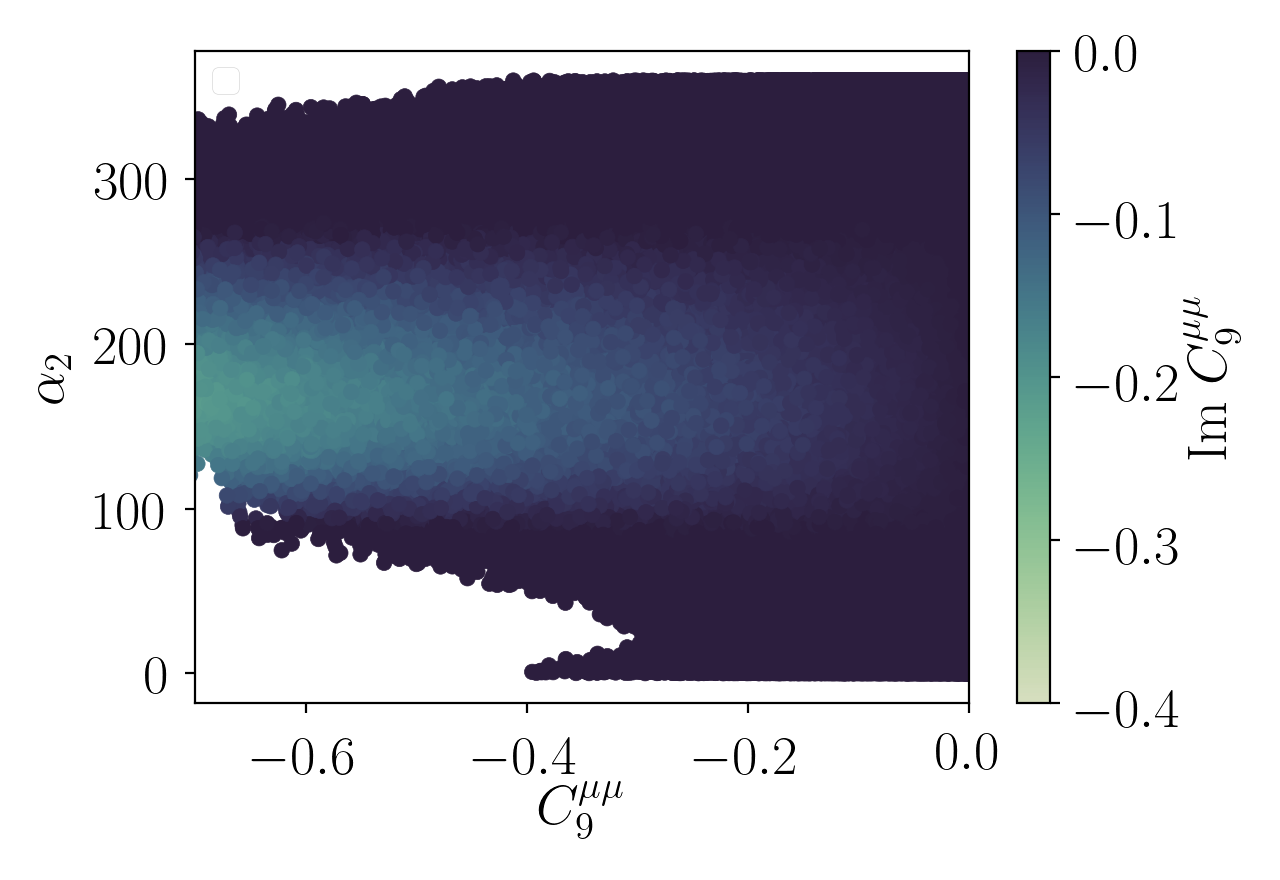
\includegraphics[width=\textwidth]{a2vsc9}
    \caption{}
    \label{fig:ch4-subfig1}
  \end{subfigure}
  \begin{subfigure}{0.495\linewidth}
    \centering
    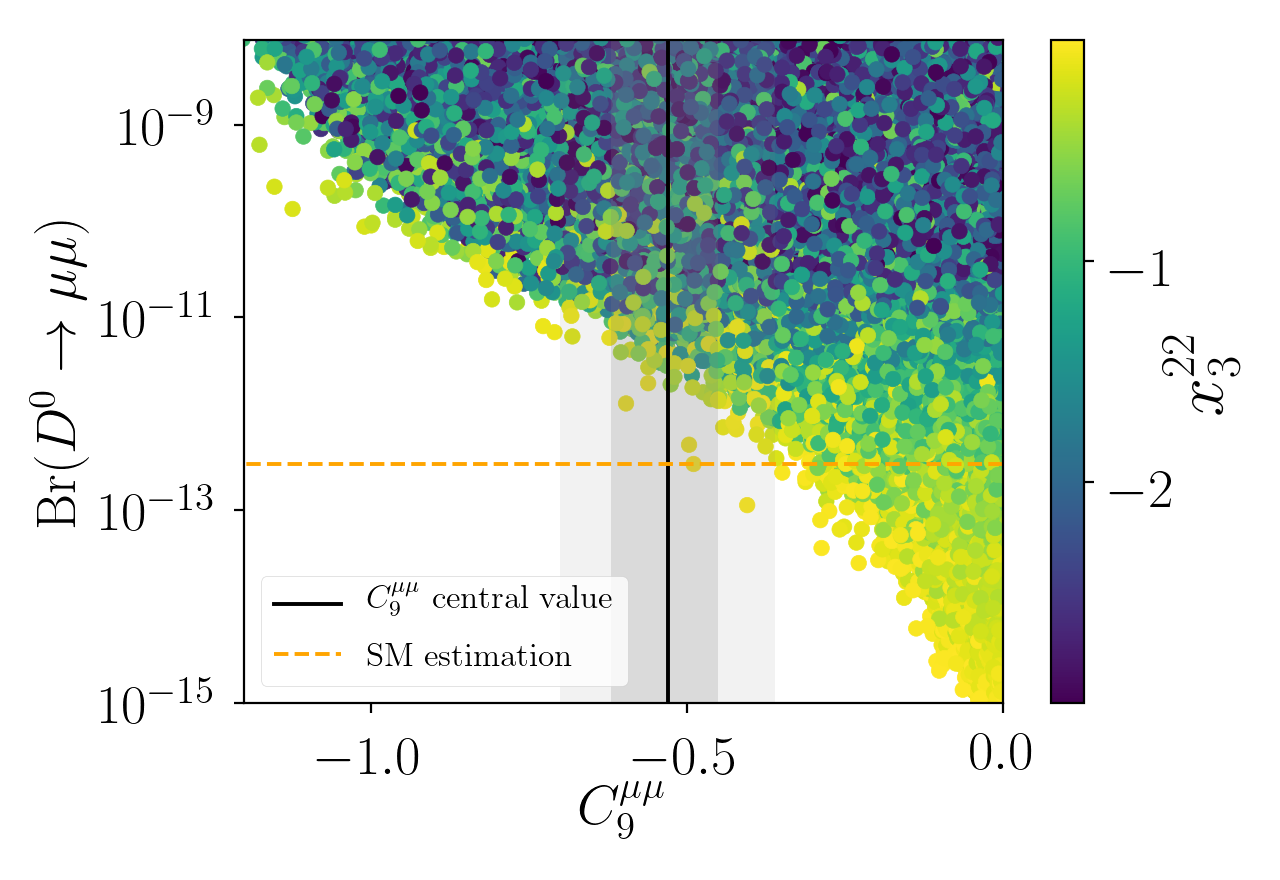
\includegraphics[width=\textwidth]{d0mmVSc9_new}
    \caption{}
    \label{fig:ch4-subfig2}
  \end{subfigure}
  \begin{subfigure}{0.497\linewidth}
    \centering
    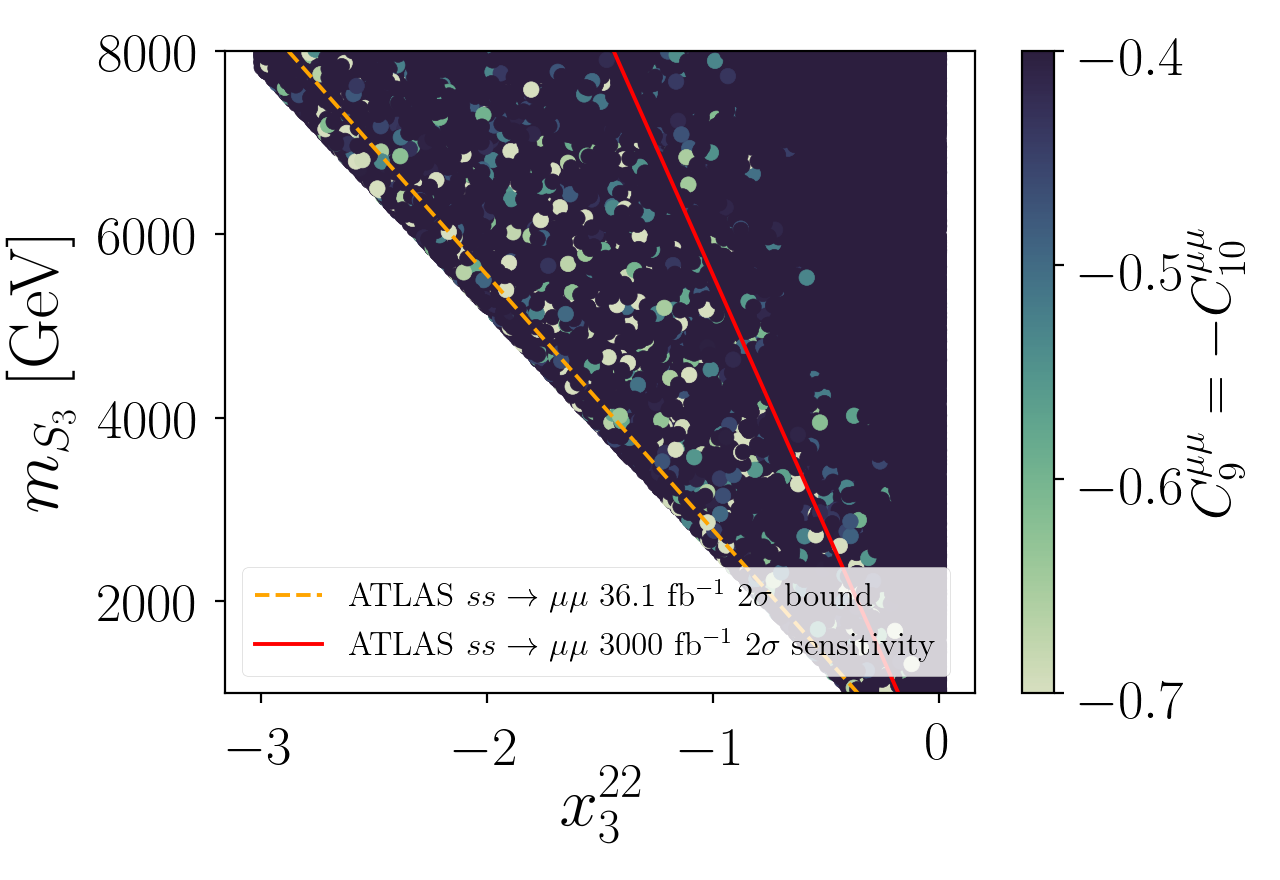
\includegraphics[width=\textwidth]{ssmmScan1_new.png}
    \caption{}
    \label{fig:ch4-subfig3}
  \end{subfigure}
  \caption[The other interesting results of our Monte Carlo analysis. (a) The
  relation between $C_{9}^{\mu\mu}$ and the Majorana phase $\alpha_{2}$. (b) The
  results of the random scan projected onto $\text{Br}(D^{0} \to \mu \mu)$ and
  $C_{9}^{\mu\mu}$.]{The other interesting results of our Monte Carlo analysis.
    (a) The relation between $C_{9}^{\mu\mu}$ and the Majorana phase
    $\alpha_{2}$. The points shown pass all of the constraints considered in our
    analysis. The colour axis represents the imaginary part of $C_{9}^{\mu\mu}$.
    The plot shows the preference away from a vanishing $\alpha_{2}$, driven by
    the constraint $\text{Br}(\mu \text{Au} \to e \text{Au})$, and the
    consistency of the available parameter space with a small imaginary part of
    $C_{9}^{\mu\mu}$. (b) The results of the random scan projected onto
    $\text{Br}(D^{0} \to \mu \mu)$ and $C_{9}^{\mu\mu}$. Points shown pass all
    constraints. Our model predicts
    $\text{Br}(D^{0} \to \mu \mu) \gtrsim 10^{-12}$, about an order of magnitude
    larger than the SM estimate from Ref.~\cite{Burdman:2001tf}. We note that
    our calculation is not valid below the dashed orange line since it only
    represents the new-physics contribution. (c) The plot shows the influence of
    the ATLAS $ss \to \mu\mu$ limits on the parameter space of our model.
    Coloured points lie in the $2\sigma$ region of the $b \to s$ fit we use.
    Dark blue points cannot explain the $b \to s$ data. The dashed orange line
    corresponds to the current ATLAS limit, while the solid red line is the
    $3000 \text{ fb}^{-1}$ projection. The abrupt absence of points in the
    bottom left of the plot is due to the constraint $D^{0} \to \mu \mu$.}
  \label{fig:ch4-otherscan1results}
\end{figure}

The leptoquark $S_{3}$ mediates highly-constraining processes of muon--electron
conversion in nuclei at tree-level, and the couplings involved are directly
related to those that explain the neutrino masses and the $b \to s$ anomalies.

We find that only about $12\%$ of the points in our numerical scan are rejected
on the basis of a constraint, but from among these almost all are disallowed
because they violate the muon--electron conversion bound given in
Table~\ref{tab:ch4-lfv-summary}. In Fig.~\ref{fig:ch4-m2ecVSc9} we present the
results of our random scan with slices through the parameter space and various
projections. We find that our model requires muon--electron conversion in Gold
nuclei at a rate no less than $2 \cdot 10^{-13}$ to accommodate the preferred
value of $C_{9}^{\mu\mu}$. The COMET~\cite{KURUP201138, Cui:2009zz, Wu:2017zwh,
  Adamov:2018vin} and Mu2e~\cite{Bartoszek:2014mya, Pezzullo:2018fzp,
  Bonventre:2019grv} experiments have projected sensitivities of
$\text{Br}(\mu \text{Al} \to e\text{Al}) \lesssim 10^{-16}$ at $90\%$
confidence\footnote{Although COMET and Mu2e will measure muon--electron
  conversion in Aluminium, we nevertheless display the result on the same plot
  since we find that the calculations in Gold and Aluminium differ by less than
  an order of magnitude.}. These will provide an improvement on the current
limit by four orders of magnitude, and will test and potentially falsify this
scenario. Interestingly, our model cannot simultaneously avoid the
muon--electron conversion bound and explain the $b \to s$ anomalies with a
vanishing Majorana phase $\alpha_{2}$, a result made clear in
Fig.~\ref{fig:ch4-subfig1}. There, it is also apparent that the constraint can
be avoided for $100^{\circ} \lesssim \alpha_{2} \lesssim 300^{\circ}$, a region
that overlaps with that shown in Fig.~\ref{fig:ch4-c9rat}, needed for a small
imaginary part for the electron couplings $x_{3}^{13}$. We find that an
additional two constraints cut into the parameter space significantly: bounds
from $D^{0} \to \mu \mu$ and the ATLAS measurement of $ss \to \mu\mu$. Our model
predicts the $D^{0} \to \mu \mu$ rate to be an order of magnitude larger than
estimates of the SM contribution
$\text{Br}(D^0 \to \mu \mu)_{\text{SM}} \sim 3 \cdot 10^{-13}$~\cite{Burdman:2001tf}
(see Fig.~\ref{fig:ch4-subfig2}), while the ATLAS $\SI{3000}{\per\fb}$
projected limit from $ss \to \mu\mu$ indicates that a non-observation would
almost entirely rule out the model for low leptoquark masses (see
Fig.~\ref{fig:ch4-subfig3}).


\subsubsection{Comments on explaining $R_{D^{(*)}}$ with the vector operator}

In our analysis above we consider only contributions in the scalar--tensor
direction to explain the charged-current anomalies in $R_D$ and $R_{D^*}$,
necessitating the inclusion of $S_{1}$ in this model to generate these
contributions. This choice is made to avoid the dangerous contributions to
$B \to K^{(*)} \nu \nu$, which necessarily exist in the presence of a large
$C_{V_L}$. We explored two ways these constraints could be avoided in the
context of our model:
\begin{enumerate}
  \item As discussed previously in the
        literature~\cite{Cai:2017wry,Deshpand:2016cpw, Altmannshofer:2017poe},
        one way to avoid the constraints from $B \to K^{(*)}\nu\nu$ and
        $B_s$--$\bar{B}_s$ mixing is to explain the $R_{D^{(*)}}$ anomalies with
        a large $x^{33}_{1}$ while ensuring $x^{32}_{1} \approx 0$. The coupling
        $z^{32}_{1}$ required to explain $R_{D^{(*)}}$ is generated through
        Eq.~\eqref{eq:ch4-z-relation}, while keeping the strange-quark coupling to
        the neutrinos zero. Combining Eq.~\eqref{eq:ch4-z-relation} and
        Eq.~\eqref{eq:ch4-cvl} with $x^{33}_{1} \gg x^{33}_{3}$ gives
    \begin{equation}
    C_{V} = \frac{\cos \theta_L}{4\sqrt{2} G_F V_{cb}} \frac{|x^{33}_{1}|^2 V_{ts}}{m_{S_{1}}^2},
    \end{equation}
        which implies
        $1.7 \lesssim |x^{33}_{1}| / (m_{S_{1}}~\TeV) \lesssim 7.2$ for
        $\cos \theta_L \approx 1$ to explain $R_{D^{(*)}}$ according to our fit
        to $C_{V}$ (see Table~\ref{tab:ch3-fitresults}). We note here that even
        saturating the lower $2\sigma$ bound on $C_{V}$ leads to contributions
        to $Z \to \tau \tau$ that disagree with experiment, despite the
        reduction of the global average driven by the latest Belle result.

  \item Ref.~\cite{Crivellin:2017zlb} proposed that the $R_{D^{(*)}}$ anomalies
        could be explained through the vector operator by considering a
        cancellation between the $S_{1}$ and $S_{3}$ particles in this model to
        the processes $B \to K^{(*)}\nu\nu$. This was further studied in
        Ref.~\cite{Buttazzo:2017ixm} and Ref.~\cite{Marzocca:2018wcf}. We have
        investigated this suggestion in considerable detail for this model, and
        could not find any parameter space that could simultaneously resolve the
        $R_{D^{(*)}}$ anomalies and be consistent with constraints from
        $B_s$--$\bar{B}_s$ mixing. Our findings are in agreement with
        Ref.~\cite{Marzocca:2018wcf}. We note that Ref.~\cite{Marzocca:2018wcf}
        proposed some lines of investigation, such as the use of complex-valued
        couplings constants, that could potentially alter this conclusion, but
        an investigation of such a scenario is beyond the scope of this study.
\end{enumerate}

\section{Radiative models explaining the flavour anomalies with leptoquarks}

The success of the non-minimal model just studied is a promising indication for
combined explanations of neutrino mass and the flavour anomalies.
Fig.~\ref{fig:ch2-scalar-piechart} suggests that the scalar leptoquarks $S_{1}$
and $S_3$, there respectively denoted $\omega_{1}$ and $\zeta$, appear often in
models of radiative neutrino mass. Indeed, the appearance of both fields
together in the non-minimal model studied above is somewhat \textit{ad hoc},
since any one leptoquark is sufficient to violate lepton number by two units in
the presence of $\chi$. It would be attractive to therefore search for radiative
models in which both $S_{1}$ and $S_{3}$ were necessary for the mechanism of
lepton-number violation. Doing so would introduce an even tighter connection
between all of the anomalies and the neutrino masses. As discussed briefly in
Sec.~\ref{sec:ch2-anomalies-mv}, the leptoquark
$R_{2} \sim (\mathbf{3}, \mathbf{2}, \tfrac{7}{6})$ can also explain the
charged-current anomalies in a relatively unconstrained way. Our analysis of the
exotics appearing in the model database indicates that it is the most common
field to appear in radiative models. Again, this is clear from
Fig.~\ref{fig:ch2-scalar-piechart}, where $R_{2}$ is denoted $\Pi_{7}$.

We search the filtered model database introduced in
Chapter~\ref{chapter:mv-models} for Lagrangians containing (i) $S_{1}$ and
$S_{3}$, or (ii) $R_{2}$ and $S_{3}$, where all of these fields are required to
couple as leptoquarks. We find 84 models for case (i) and 203 models for case
(ii). All of the models are derived from dimension-eleven operators and contain
more than three exotic fields, with the exception of four of the $R_{2} + S_{3}$
models that require only one more scalar to violate lepton number. These models
are summaried in Table~\ref{tab:ch4-minimal-mv-table}, along with a small random
sample from the remaining 283 models of cases (i) and (ii). The models tend to
imply a large upper bound on the new-physics scale, since the operators from
which they are derived tend to contain two $L$ fields. This reduces the number
of loops and SM-lepton mass insertions required in the operator closure. Models
in which $S_{1}$ or $R_{2}$ couple to $\bar{e}$ instead of $L$ are in general
filtered out by those models in which the leptoquark couplings to $L$ feature in
the $\Delta L = 2$ mechanism. This phenomenon is also seen and discussed in
Sec.~\ref{sec:ch2-anomalies-mv}.

\begin{table}
  \centering
  \bgroup
  \def\arraystretch{1.3}
  \begin{tabular}{ccl}
    \toprule
    $S_{3} + \text{field content} $ & Operators & $\Lambda~[\TeV]$ \\
    \midrule
    $R_{2}$, $(\mathbf{3}, \mathbf{1}, \tfrac{2}{3})_{S}$ & $71$ & $2 \cdot 10^{7}$ \\
    $R_{2}$, $(\mathbf{3}, \mathbf{3}, \tfrac{2}{3})_{S}$ & $71$ & $2 \cdot 10^{7}$ \\
    $R_{2}$, $(\mathbf{3}, \mathbf{4}, \tfrac{1}{6})_{S}$ & $71$ & $2 \cdot 10^{7}$ \\
    $R_{2}$, $(\mathbf{1}, \mathbf{4}, \tfrac{3}{2})_{S}$ & $71$ & $2 \cdot 10^{7}$ \\
    $R_{2}$, $(\mathbf{8}, \mathbf{1}, 1)_{S}$, $(\mathbf{3}, \mathbf{1}, \tfrac{2}{3})_{F}$ & $25c$ & $4 \cdot 10^{3}$ \\
    $R_{2}$, $(\mathbf{8}, \mathbf{3}, 1)_{S}$, $(\mathbf{3}, \mathbf{3}, \tfrac{2}{3})_{F}$ & $25c$ & $4 \cdot 10^{3}$ \\
    $R_{2}$, $(\mathbf{8}, \mathbf{2}, \tfrac{1}{2})_{F}$, $(\mathbf{8}, \mathbf{3}, 0)_{F}$ & $29c$ & $2 \cdot 10^{7}$ \\
    $S_{1}$, $(\mathbf{3}, \mathbf{2}, \tfrac{1}{6})_{F}$, $(\bar{\mathbf{6}}, \mathbf{2}, \tfrac{1}{6})_{S}$ & $25c$ & $4 \cdot 10^{3}$ \\
    $S_{1}$, $(\mathbf{\bar{3}}, \mathbf{3}, \tfrac{1}{3})_{F}$, $(\mathbf{\bar{6}}, \mathbf{3}, \tfrac{2}{3})_{S}$ & $47i$ & $2 \cdot 10^{7}$ \\
    $S_{1}$, $(\mathbf{3}, \mathbf{3}, \tfrac{2}{3})_{S}$, $(\mathbf{3}, \mathbf{4}, \tfrac{1}{6})_{F}$ & $40h$ & $2 \cdot 10^{7}$ \\
    \bottomrule
  \end{tabular}
  \egroup
  \caption[The table shows a small sample of the 287 models of radiative
  neutrino mass that also contain either both of $S_{3}$ and $R_{2}$ or both of
  $S_{3}$ and $S_{1}$.]{The table shows a small sample of the 287 models of
    radiative neutrino mass that also contain either both of $S_{3}$ and $R_{2}$
    or both of $S_{3}$ and $S_{1}$. The first four models listed are the only
    ones of the 287 that contain only three fields in total. The models tend to
    have a high predicted scale since two $L$ fields are generally present in
    the operators, reducing the number of loops and SM-lepton mass insertions
    required in the operator closure.}
  \label{tab:ch4-minimal-mv-table}
\end{table}


\section{Conclusions}

In this chapter we have begun to explore the connection between models of
radiative neutrino mass and explanations of the flavour anomalies. We did this
by first taking the BN scenario and embedding it into a simple two-loop model,
first studied in Ref.~\cite{Angel:2013hla}, from the model database studied in
Chapter~\ref{chapter:mv-models}. The tight connection between the neutrino-mass
generation and the explanation of the anomalies means that the model cannot
simultaneously explain the neutrino masses and the $b \to s$ data on account of
$\tau \to \mu$ and $\mu \to e$ LFV observables. Specifically, bounds from
muon--electron conversion in nuclei fix the ratio of the couplings $x_{33}$ and
$x_{23}$ in the $S_{1}$ model, so that the large value of $x_{23}$ required to
generate $C_{LL} \approx -1$ (see Eq.~\eqref{eq:ch3-rknncond}) leads to
$\tau \to \mu \gamma$ and $\tau \to \mu\mu\mu$ rates incompatible with
experiment. The fixing of $x_{33} / x_{23}$ in this model is ultimately due to
the fact that the coupling of $S_{1}$ to the electron cannot be avoided in the
neutrino-mass model, and the structure of the mass matrix is such that one can
ensure $x_{13} \approx 0$ at the cost of fixing $x_{33} / x_{23}$.

To address the limited success of this neutrino-mass model, we also studied a
non-minimal scenario containing the leptoquark $S_{3}$ in addition to $S_{1}$.
Here, we were mainly interested in the extent to which bounds from
muon--electron conversion could accommodate an explanation of the flavour
anomalies in a neutrino-mass model. Although the $S_{3}$ explanation of the
$b \to s$ anomalies is usually relatively unconstrained, introducing the
neutrino-mass connection leads to a rich phenomenology wherein a value of
$C_{LL}$ compatible with an explanation of the neutral-current anomalies
requires a muon--electron conversion rate in Gold nuclei of no less than
$2 \cdot 10^{-13}$, within reach of the upcoming COMET and Mu2e experiments. The
model also predicts a range for the Majorana phase $\alpha_{2}$ of
$100^{\circ} \lesssim \alpha_{2} \lesssim 300^{\circ}$, and a rate for
$D^{0} \to \mu\mu$ an order of magnitude larger than the SM value.

The $S_{1} + S_{3}$ model can successfully explain all of the flavour anomalies
to within $1\sigma$, while respecting all of the constraints we consider in our
analysis. The model is non-minimal both in the sense that two fields explain the
anomalies separately, but also in the sense that both of these fields are not
necessary for lepton-number violation. A tighter connection between the neutrino
mass and the flavour anomalies may be seen in a model in which all of the exotic
multiplets play some role in the violation of lepton number. We find 287 such
models that explain the $b \to s$ anomalies with $S_{3}$ and the $b \to c$
anomalies with one of $S_{1}$ or $R_{2}$. There are four $S_{3} + R_{2}$ models
that contain only three exotic fields in total. From here the stage is set for a
fuller exploration of these models and the exciting predictions they may imply
for both neutrino and flavour physics.
